\documentclass[twoside]{book}

% Packages required by doxygen
\usepackage{fixltx2e}
\usepackage{calc}
\usepackage{doxygen}
\usepackage[export]{adjustbox} % also loads graphicx
\usepackage{graphicx}
\usepackage[utf8]{inputenc}
\usepackage{makeidx}
\usepackage{multicol}
\usepackage{multirow}
\PassOptionsToPackage{warn}{textcomp}
\usepackage{textcomp}
\usepackage[nointegrals]{wasysym}
\usepackage[table]{xcolor}

% Font selection
\usepackage[T1]{fontenc}
\usepackage[scaled=.90]{helvet}
\usepackage{courier}
\usepackage{amssymb}
\usepackage{sectsty}
\renewcommand{\familydefault}{\sfdefault}
\allsectionsfont{%
  \fontseries{bc}\selectfont%
  \color{darkgray}%
}
\renewcommand{\DoxyLabelFont}{%
  \fontseries{bc}\selectfont%
  \color{darkgray}%
}
\newcommand{\+}{\discretionary{\mbox{\scriptsize$\hookleftarrow$}}{}{}}

% Page & text layout
\usepackage{geometry}
\geometry{%
  a4paper,%
  top=2.5cm,%
  bottom=2.5cm,%
  left=2.5cm,%
  right=2.5cm%
}
\tolerance=750
\hfuzz=15pt
\hbadness=750
\setlength{\emergencystretch}{15pt}
\setlength{\parindent}{0cm}
\setlength{\parskip}{3ex plus 2ex minus 2ex}
\makeatletter
\renewcommand{\paragraph}{%
  \@startsection{paragraph}{4}{0ex}{-1.0ex}{1.0ex}{%
    \normalfont\normalsize\bfseries\SS@parafont%
  }%
}
\renewcommand{\subparagraph}{%
  \@startsection{subparagraph}{5}{0ex}{-1.0ex}{1.0ex}{%
    \normalfont\normalsize\bfseries\SS@subparafont%
  }%
}
\makeatother

% Headers & footers
\usepackage{fancyhdr}
\pagestyle{fancyplain}
\fancyhead[LE]{\fancyplain{}{\bfseries\thepage}}
\fancyhead[CE]{\fancyplain{}{}}
\fancyhead[RE]{\fancyplain{}{\bfseries\leftmark}}
\fancyhead[LO]{\fancyplain{}{\bfseries\rightmark}}
\fancyhead[CO]{\fancyplain{}{}}
\fancyhead[RO]{\fancyplain{}{\bfseries\thepage}}
\fancyfoot[LE]{\fancyplain{}{}}
\fancyfoot[CE]{\fancyplain{}{}}
\fancyfoot[RE]{\fancyplain{}{\bfseries\scriptsize Generated by Doxygen }}
\fancyfoot[LO]{\fancyplain{}{\bfseries\scriptsize Generated by Doxygen }}
\fancyfoot[CO]{\fancyplain{}{}}
\fancyfoot[RO]{\fancyplain{}{}}
\renewcommand{\footrulewidth}{0.4pt}
\renewcommand{\chaptermark}[1]{%
  \markboth{#1}{}%
}
\renewcommand{\sectionmark}[1]{%
  \markright{\thesection\ #1}%
}

% Indices & bibliography
\usepackage{natbib}
\usepackage[titles]{tocloft}
\setcounter{tocdepth}{3}
\setcounter{secnumdepth}{5}
\makeindex

% Hyperlinks (required, but should be loaded last)
\usepackage{ifpdf}
\ifpdf
  \usepackage[pdftex,pagebackref=true]{hyperref}
\else
  \usepackage[ps2pdf,pagebackref=true]{hyperref}
\fi
\hypersetup{%
  colorlinks=true,%
  linkcolor=blue,%
  citecolor=blue,%
  unicode%
}

% Custom commands
\newcommand{\clearemptydoublepage}{%
  \newpage{\pagestyle{empty}\cleardoublepage}%
}

\usepackage{caption}
\captionsetup{labelsep=space,justification=centering,font={bf},singlelinecheck=off,skip=4pt,position=top}

%===== C O N T E N T S =====

\begin{document}

% Titlepage & ToC
\hypersetup{pageanchor=false,
             bookmarksnumbered=true,
             pdfencoding=unicode
            }
\pagenumbering{roman}
\begin{titlepage}
\vspace*{7cm}
\begin{center}%
{\Large 05.print\+\_\+ip }\\
\vspace*{1cm}
{\large Generated by Doxygen 1.8.11}\\
\end{center}
\end{titlepage}
\clearemptydoublepage
\tableofcontents
\clearemptydoublepage
\pagenumbering{arabic}
\hypersetup{pageanchor=true}

%--- Begin generated contents ---
\chapter{Hierarchical Index}
\section{Class Hierarchy}
This inheritance list is sorted roughly, but not completely, alphabetically\+:\begin{DoxyCompactList}
\item false\+\_\+type\begin{DoxyCompactList}
\item \contentsline{section}{is\+\_\+specialization\+\_\+of$<$ Template, T $>$}{\pageref{structis__specialization__of}}{}
\end{DoxyCompactList}
\item \contentsline{section}{Ip\+Printer\+Base$<$ Derived $>$}{\pageref{struct_ip_printer_base}}{}
\item \contentsline{section}{Ip\+Printer\+Base$<$ Ip\+Printer $>$}{\pageref{struct_ip_printer_base}}{}
\begin{DoxyCompactList}
\item \contentsline{section}{Ip\+Printer}{\pageref{class_ip_printer}}{}
\end{DoxyCompactList}
\item \contentsline{section}{Logger}{\pageref{struct_logger}}{}
\item true\+\_\+type\begin{DoxyCompactList}
\item \contentsline{section}{is\+\_\+specialization\+\_\+of$<$ Template, Template$<$ Args... $>$ $>$}{\pageref{structis__specialization__of_3_01_template_00_01_template_3_01_args_8_8_8_01_4_01_4}}{}
\end{DoxyCompactList}
\end{DoxyCompactList}

\chapter{Class Index}
\section{Class List}
Here are the classes, structs, unions and interfaces with brief descriptions\+:\begin{DoxyCompactList}
\item\contentsline{section}{\hyperlink{structis__specialization__of}{is\+\_\+specialization\+\_\+of$<$ Template, T $>$} }{\pageref{structis__specialization__of}}{}
\item\contentsline{section}{\hyperlink{structis__specialization__of_3_01_template_00_01_template_3_01_args_8_8_8_01_4_01_4}{is\+\_\+specialization\+\_\+of$<$ Template, Template$<$ Args... $>$ $>$} }{\pageref{structis__specialization__of_3_01_template_00_01_template_3_01_args_8_8_8_01_4_01_4}}{}
\item\contentsline{section}{\hyperlink{struct_logger}{Logger} }{\pageref{struct_logger}}{}
\end{DoxyCompactList}

\chapter{File Index}
\section{File List}
Here is a list of all files with brief descriptions\+:\begin{DoxyCompactList}
\item\contentsline{section}{\hyperlink{logger_8h}{logger.\+h} }{\pageref{logger_8h}}{}
\item\contentsline{section}{\hyperlink{main_8cpp}{main.\+cpp} }{\pageref{main_8cpp}}{}
\item\contentsline{section}{\hyperlink{print__ip_8h}{print\+\_\+ip.\+h} }{\pageref{print__ip_8h}}{}
\item\contentsline{section}{\hyperlink{share_8h}{share.\+h} }{\pageref{share_8h}}{}
\item\contentsline{section}{\hyperlink{tests_8cpp}{tests.\+cpp} }{\pageref{tests_8cpp}}{}
\end{DoxyCompactList}

\chapter{Class Documentation}
\hypertarget{class_ip_printer}{}\section{Ip\+Printer Class Reference}
\label{class_ip_printer}\index{Ip\+Printer@{Ip\+Printer}}


{\ttfamily \#include $<$print\+\_\+ip.\+h$>$}



Inheritance diagram for Ip\+Printer\+:
\nopagebreak
\begin{figure}[H]
\begin{center}
\leavevmode
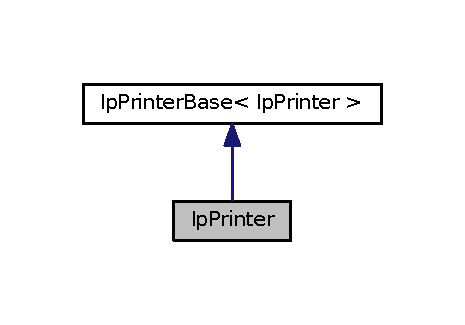
\includegraphics[width=223pt]{class_ip_printer__inherit__graph}
\end{center}
\end{figure}


Collaboration diagram for Ip\+Printer\+:
\nopagebreak
\begin{figure}[H]
\begin{center}
\leavevmode
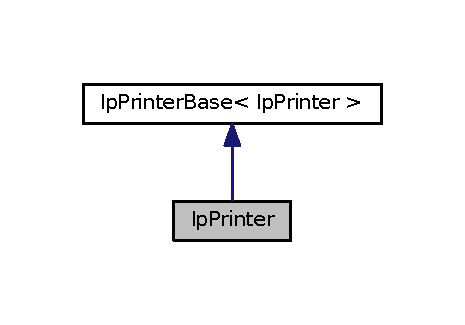
\includegraphics[width=223pt]{class_ip_printer__coll__graph}
\end{center}
\end{figure}
\subsection*{Friends}
\begin{DoxyCompactItemize}
\item 
struct \hyperlink{class_ip_printer_a75f196212357865a0588d194fb42d17c}{Ip\+Printer\+Base$<$ Ip\+Printer $>$}
\end{DoxyCompactItemize}
\subsection*{Additional Inherited Members}


\subsection{Detailed Description}


Definition at line 56 of file print\+\_\+ip.\+h.



\subsection{Friends And Related Function Documentation}
\index{Ip\+Printer@{Ip\+Printer}!Ip\+Printer\+Base$<$ Ip\+Printer $>$@{Ip\+Printer\+Base$<$ Ip\+Printer $>$}}
\index{Ip\+Printer\+Base$<$ Ip\+Printer $>$@{Ip\+Printer\+Base$<$ Ip\+Printer $>$}!Ip\+Printer@{Ip\+Printer}}
\subsubsection[{\texorpdfstring{Ip\+Printer\+Base$<$ Ip\+Printer $>$}{IpPrinterBase< IpPrinter >}}]{\setlength{\rightskip}{0pt plus 5cm}friend struct {\bf Ip\+Printer\+Base}$<$ {\bf Ip\+Printer} $>$\hspace{0.3cm}{\ttfamily [friend]}}\hypertarget{class_ip_printer_a75f196212357865a0588d194fb42d17c}{}\label{class_ip_printer_a75f196212357865a0588d194fb42d17c}


Definition at line 57 of file print\+\_\+ip.\+h.



The documentation for this class was generated from the following file\+:\begin{DoxyCompactItemize}
\item 
\hyperlink{print__ip_8h}{print\+\_\+ip.\+h}\end{DoxyCompactItemize}

\hypertarget{struct_ip_printer_base}{}\section{Ip\+Printer\+Base$<$ Derived $>$ Struct Template Reference}
\label{struct_ip_printer_base}\index{Ip\+Printer\+Base$<$ Derived $>$@{Ip\+Printer\+Base$<$ Derived $>$}}


{\ttfamily \#include $<$print\+\_\+ip.\+h$>$}

\subsection*{Public Member Functions}
\begin{DoxyCompactItemize}
\item 
{\footnotesize template$<$typename T $>$ }\\string \hyperlink{struct_ip_printer_base_a598e5b30fdaf6e24a099cd2eea8eeddf}{print\+\_\+ip\+\_\+from\+\_\+numeric} (const T \&ip)
\item 
{\footnotesize template$<$typename Arg , typename... Args$>$ }\\string \hyperlink{struct_ip_printer_base_a0f19d29526c1d6ba5e0a7ec5eee011b1}{print\+\_\+ip\+\_\+from\+\_\+tuple} (const std\+::tuple$<$ Arg, Args... $>$ \&ip)
\item 
{\footnotesize template$<$typename Container $>$ }\\string \hyperlink{struct_ip_printer_base_a8b20f00707051af8fed2254c61e8a823}{print\+\_\+ip\+\_\+from\+\_\+container} (const Container \&collect, bool b\+\_\+reverse=false)
\end{DoxyCompactItemize}


\subsection{Detailed Description}
\subsubsection*{template$<$typename Derived$>$\\*
struct Ip\+Printer\+Base$<$ Derived $>$}



Definition at line 39 of file print\+\_\+ip.\+h.



\subsection{Member Function Documentation}
\index{Ip\+Printer\+Base@{Ip\+Printer\+Base}!print\+\_\+ip\+\_\+from\+\_\+container@{print\+\_\+ip\+\_\+from\+\_\+container}}
\index{print\+\_\+ip\+\_\+from\+\_\+container@{print\+\_\+ip\+\_\+from\+\_\+container}!Ip\+Printer\+Base@{Ip\+Printer\+Base}}
\subsubsection[{\texorpdfstring{print\+\_\+ip\+\_\+from\+\_\+container(const Container \&collect, bool b\+\_\+reverse=false)}{print_ip_from_container(const Container &collect, bool b_reverse=false)}}]{\setlength{\rightskip}{0pt plus 5cm}template$<$typename Derived$>$ template$<$typename Container $>$ string {\bf Ip\+Printer\+Base}$<$ Derived $>$\+::print\+\_\+ip\+\_\+from\+\_\+container (
\begin{DoxyParamCaption}
\item[{const Container \&}]{collect, }
\item[{bool}]{b\+\_\+reverse = {\ttfamily false}}
\end{DoxyParamCaption}
)\hspace{0.3cm}{\ttfamily [inline]}}\hypertarget{struct_ip_printer_base_a8b20f00707051af8fed2254c61e8a823}{}\label{struct_ip_printer_base_a8b20f00707051af8fed2254c61e8a823}


Definition at line 51 of file print\+\_\+ip.\+h.



Here is the caller graph for this function\+:
\nopagebreak
\begin{figure}[H]
\begin{center}
\leavevmode
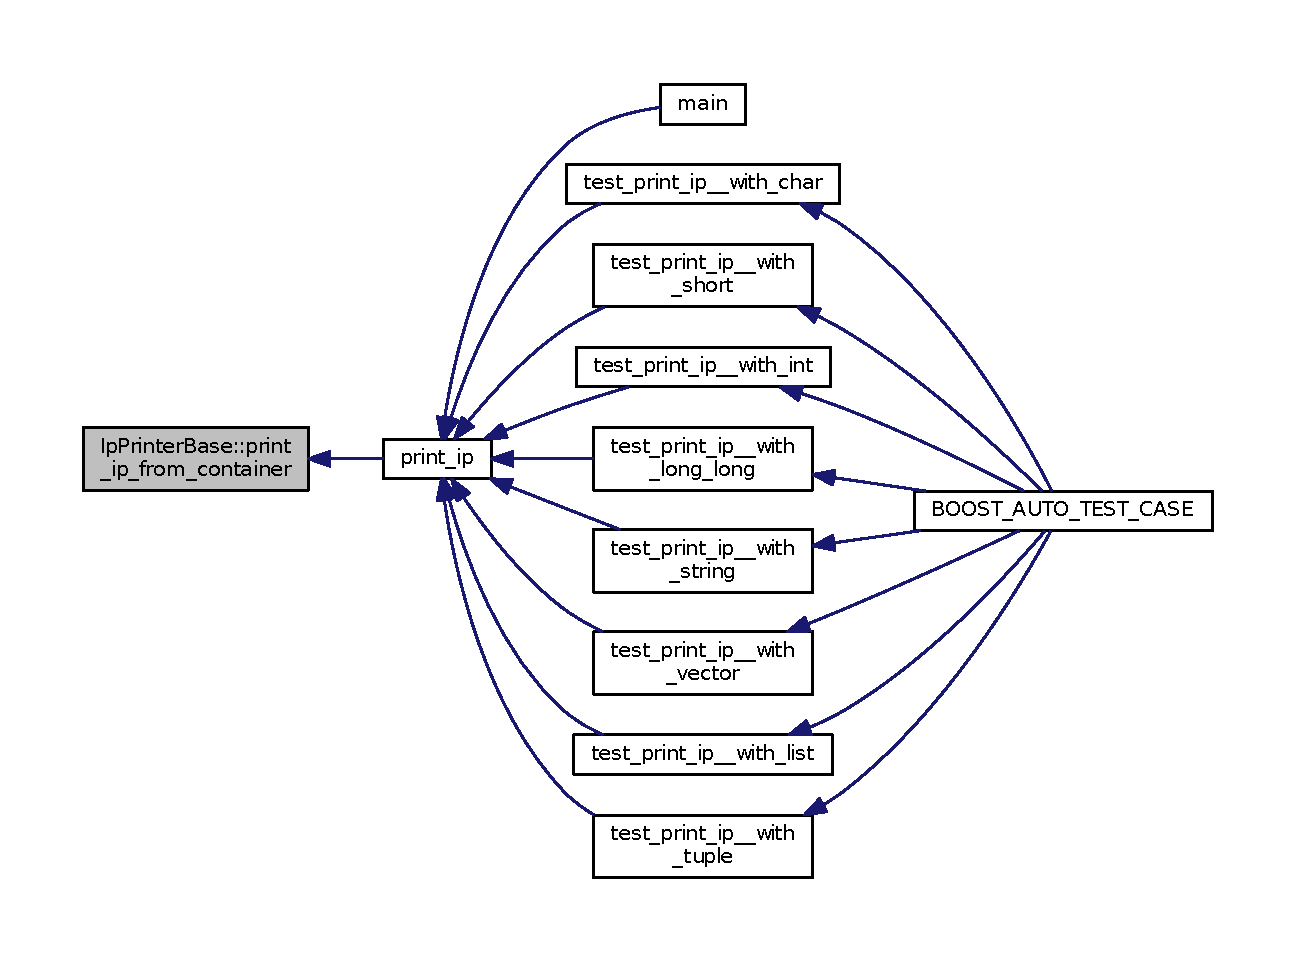
\includegraphics[width=350pt]{struct_ip_printer_base_a8b20f00707051af8fed2254c61e8a823_icgraph}
\end{center}
\end{figure}


\index{Ip\+Printer\+Base@{Ip\+Printer\+Base}!print\+\_\+ip\+\_\+from\+\_\+numeric@{print\+\_\+ip\+\_\+from\+\_\+numeric}}
\index{print\+\_\+ip\+\_\+from\+\_\+numeric@{print\+\_\+ip\+\_\+from\+\_\+numeric}!Ip\+Printer\+Base@{Ip\+Printer\+Base}}
\subsubsection[{\texorpdfstring{print\+\_\+ip\+\_\+from\+\_\+numeric(const T \&ip)}{print_ip_from_numeric(const T &ip)}}]{\setlength{\rightskip}{0pt plus 5cm}template$<$typename Derived$>$ template$<$typename T $>$ string {\bf Ip\+Printer\+Base}$<$ Derived $>$\+::print\+\_\+ip\+\_\+from\+\_\+numeric (
\begin{DoxyParamCaption}
\item[{const T \&}]{ip}
\end{DoxyParamCaption}
)\hspace{0.3cm}{\ttfamily [inline]}}\hypertarget{struct_ip_printer_base_a598e5b30fdaf6e24a099cd2eea8eeddf}{}\label{struct_ip_printer_base_a598e5b30fdaf6e24a099cd2eea8eeddf}


Definition at line 41 of file print\+\_\+ip.\+h.



Here is the caller graph for this function\+:
\nopagebreak
\begin{figure}[H]
\begin{center}
\leavevmode
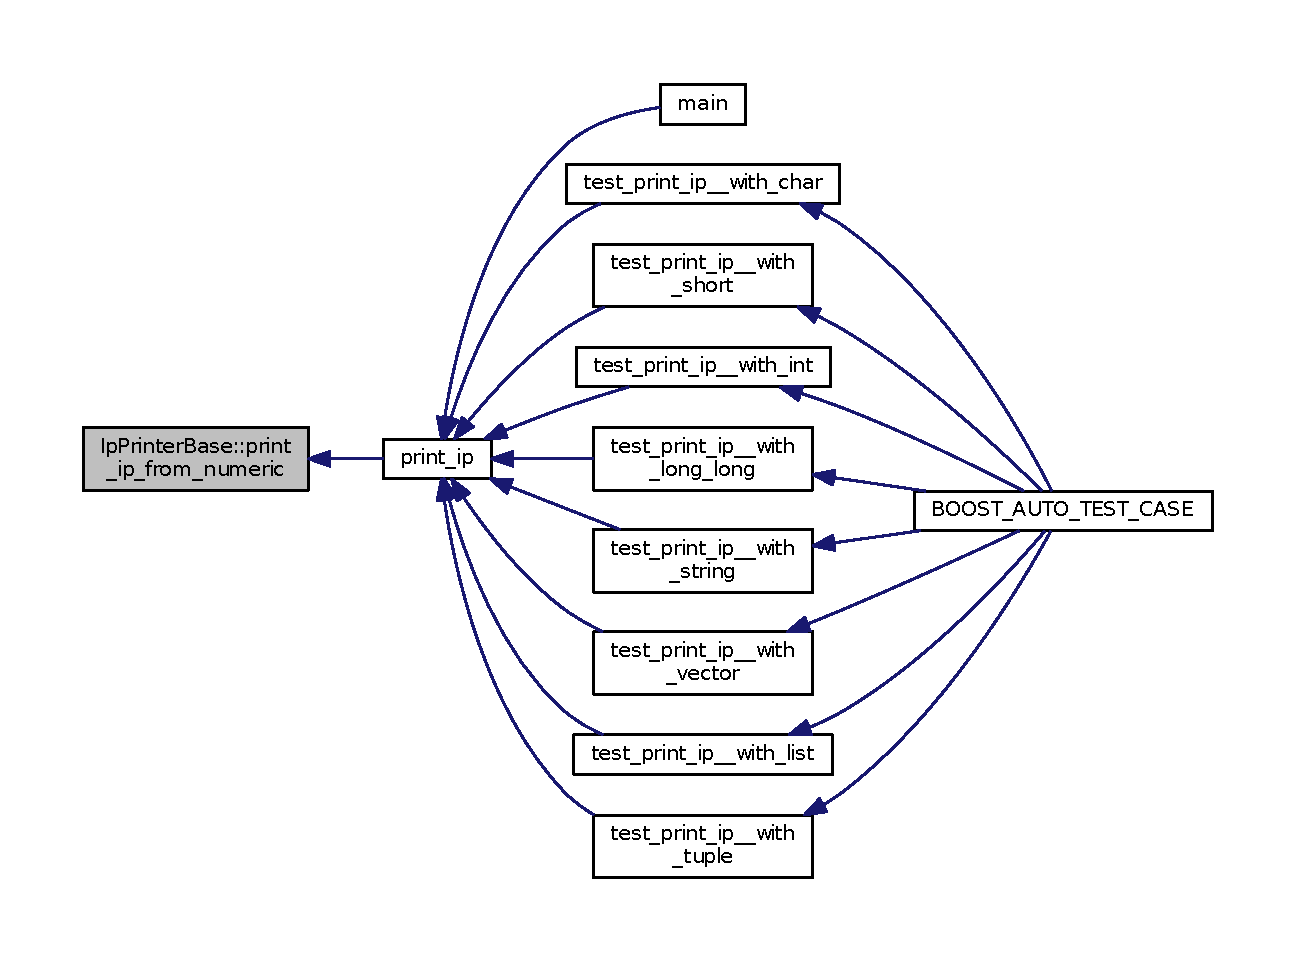
\includegraphics[width=350pt]{struct_ip_printer_base_a598e5b30fdaf6e24a099cd2eea8eeddf_icgraph}
\end{center}
\end{figure}


\index{Ip\+Printer\+Base@{Ip\+Printer\+Base}!print\+\_\+ip\+\_\+from\+\_\+tuple@{print\+\_\+ip\+\_\+from\+\_\+tuple}}
\index{print\+\_\+ip\+\_\+from\+\_\+tuple@{print\+\_\+ip\+\_\+from\+\_\+tuple}!Ip\+Printer\+Base@{Ip\+Printer\+Base}}
\subsubsection[{\texorpdfstring{print\+\_\+ip\+\_\+from\+\_\+tuple(const std\+::tuple$<$ Arg, Args... $>$ \&ip)}{print_ip_from_tuple(const std::tuple< Arg, Args... > &ip)}}]{\setlength{\rightskip}{0pt plus 5cm}template$<$typename Derived$>$ template$<$typename Arg , typename... Args$>$ string {\bf Ip\+Printer\+Base}$<$ Derived $>$\+::print\+\_\+ip\+\_\+from\+\_\+tuple (
\begin{DoxyParamCaption}
\item[{const std\+::tuple$<$ Arg, Args... $>$ \&}]{ip}
\end{DoxyParamCaption}
)\hspace{0.3cm}{\ttfamily [inline]}}\hypertarget{struct_ip_printer_base_a0f19d29526c1d6ba5e0a7ec5eee011b1}{}\label{struct_ip_printer_base_a0f19d29526c1d6ba5e0a7ec5eee011b1}


Definition at line 46 of file print\+\_\+ip.\+h.



Here is the caller graph for this function\+:
\nopagebreak
\begin{figure}[H]
\begin{center}
\leavevmode
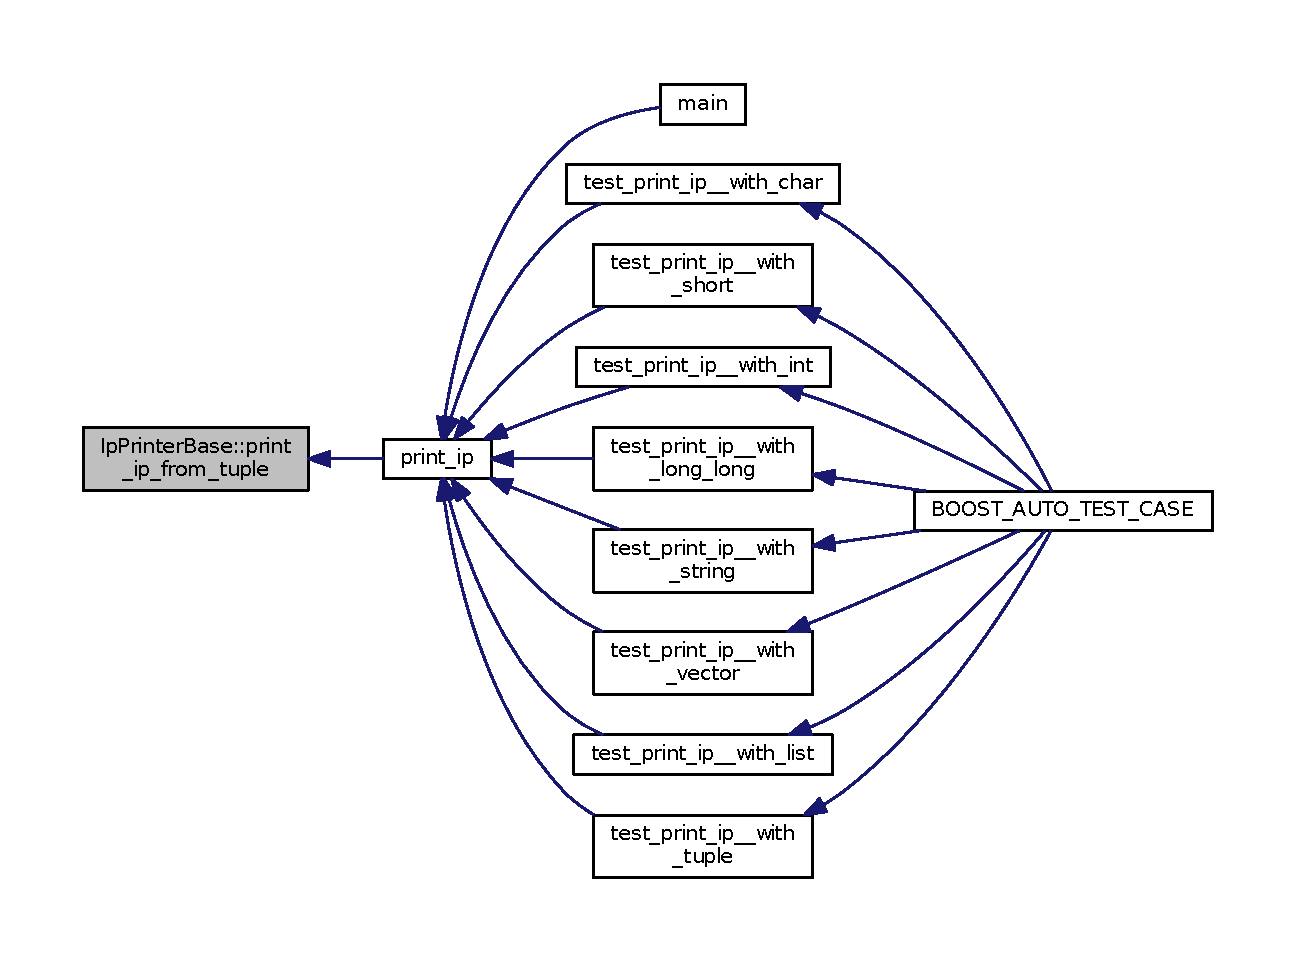
\includegraphics[width=350pt]{struct_ip_printer_base_a0f19d29526c1d6ba5e0a7ec5eee011b1_icgraph}
\end{center}
\end{figure}




The documentation for this struct was generated from the following file\+:\begin{DoxyCompactItemize}
\item 
\hyperlink{print__ip_8h}{print\+\_\+ip.\+h}\end{DoxyCompactItemize}

\hypertarget{structis__specialization__of}{}\section{is\+\_\+specialization\+\_\+of$<$ Template, T $>$ Struct Template Reference}
\label{structis__specialization__of}\index{is\+\_\+specialization\+\_\+of$<$ Template, T $>$@{is\+\_\+specialization\+\_\+of$<$ Template, T $>$}}


{\ttfamily \#include $<$print\+\_\+ip.\+h$>$}



Inheritance diagram for is\+\_\+specialization\+\_\+of$<$ Template, T $>$\+:
\nopagebreak
\begin{figure}[H]
\begin{center}
\leavevmode
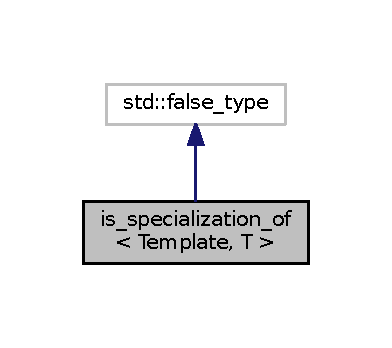
\includegraphics[width=188pt]{structis__specialization__of__inherit__graph}
\end{center}
\end{figure}


Collaboration diagram for is\+\_\+specialization\+\_\+of$<$ Template, T $>$\+:
\nopagebreak
\begin{figure}[H]
\begin{center}
\leavevmode
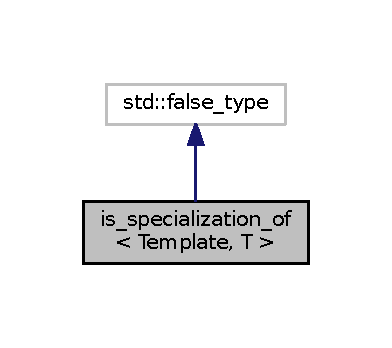
\includegraphics[width=188pt]{structis__specialization__of__coll__graph}
\end{center}
\end{figure}


\subsection{Detailed Description}
\subsubsection*{template$<$template$<$ typename... $>$ class Template, typename T$>$\\*
struct is\+\_\+specialization\+\_\+of$<$ Template, T $>$}



Definition at line 23 of file print\+\_\+ip.\+h.



The documentation for this struct was generated from the following file\+:\begin{DoxyCompactItemize}
\item 
\hyperlink{print__ip_8h}{print\+\_\+ip.\+h}\end{DoxyCompactItemize}

\hypertarget{structis__specialization__of_3_01_template_00_01_template_3_01_args_8_8_8_01_4_01_4}{}\section{is\+\_\+specialization\+\_\+of$<$ Template, Template$<$ Args... $>$ $>$ Struct Template Reference}
\label{structis__specialization__of_3_01_template_00_01_template_3_01_args_8_8_8_01_4_01_4}\index{is\+\_\+specialization\+\_\+of$<$ Template, Template$<$ Args... $>$ $>$@{is\+\_\+specialization\+\_\+of$<$ Template, Template$<$ Args... $>$ $>$}}


{\ttfamily \#include $<$print\+\_\+ip.\+h$>$}



Inheritance diagram for is\+\_\+specialization\+\_\+of$<$ Template, Template$<$ Args... $>$ $>$\+:
\nopagebreak
\begin{figure}[H]
\begin{center}
\leavevmode
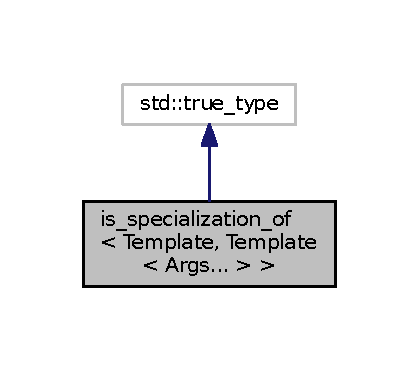
\includegraphics[width=201pt]{structis__specialization__of_3_01_template_00_01_template_3_01_args_8_8_8_01_4_01_4__inherit__graph}
\end{center}
\end{figure}


Collaboration diagram for is\+\_\+specialization\+\_\+of$<$ Template, Template$<$ Args... $>$ $>$\+:
\nopagebreak
\begin{figure}[H]
\begin{center}
\leavevmode
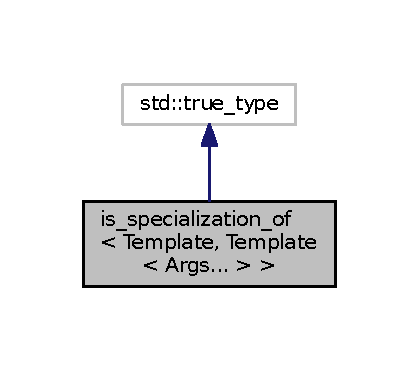
\includegraphics[width=201pt]{structis__specialization__of_3_01_template_00_01_template_3_01_args_8_8_8_01_4_01_4__coll__graph}
\end{center}
\end{figure}


\subsection{Detailed Description}
\subsubsection*{template$<$template$<$ typename... $>$ class Template, typename... Args$>$\\*
struct is\+\_\+specialization\+\_\+of$<$ Template, Template$<$ Args... $>$ $>$}



Definition at line 26 of file print\+\_\+ip.\+h.



The documentation for this struct was generated from the following file\+:\begin{DoxyCompactItemize}
\item 
\hyperlink{print__ip_8h}{print\+\_\+ip.\+h}\end{DoxyCompactItemize}

\hypertarget{struct_logger}{}\section{Logger Struct Reference}
\label{struct_logger}\index{Logger@{Logger}}


{\ttfamily \#include $<$logger.\+h$>$}

\subsection*{Public Member Functions}
\begin{DoxyCompactItemize}
\item 
\hyperlink{struct_logger_a776f6fc22d153935ab08504255f8d45c}{Logger} (\mbox{[}\mbox{[}maybe\+\_\+unused\mbox{]}\mbox{]} ostream \&out=std\+::cout, std\+::string prefix=\char`\"{}\char`\"{}, std\+::string suffix=\char`\"{}\char`\"{}, std\+::string ending=\char`\"{}\char`\"{})
\item 
{\footnotesize template$<$typename Arg , typename... Args$>$ }\\void \hyperlink{struct_logger_a5bbacf5d9e8194384faec5d5a0dd1b70}{operator()} (Arg arg, Args \&\&...args)
\end{DoxyCompactItemize}


\subsection{Detailed Description}


Definition at line 16 of file logger.\+h.



\subsection{Constructor \& Destructor Documentation}
\index{Logger@{Logger}!Logger@{Logger}}
\index{Logger@{Logger}!Logger@{Logger}}
\subsubsection[{\texorpdfstring{Logger([[maybe\+\_\+unused]] ostream \&out=std\+::cout, std\+::string prefix="""", std\+::string suffix="""", std\+::string ending="""")}{Logger([[maybe_unused]] ostream &out=std::cout, std::string prefix="", std::string suffix="", std::string ending="")}}]{\setlength{\rightskip}{0pt plus 5cm}Logger\+::\+Logger (
\begin{DoxyParamCaption}
\item[{\mbox{[}\mbox{[}maybe\+\_\+unused\mbox{]} \mbox{]} ostream \&}]{out = {\ttfamily std\+:\+:cout}, }
\item[{std\+::string}]{prefix = {\ttfamily \char`\"{}\char`\"{}}, }
\item[{std\+::string}]{suffix = {\ttfamily \char`\"{}\char`\"{}}, }
\item[{std\+::string}]{ending = {\ttfamily \char`\"{}\char`\"{}}}
\end{DoxyParamCaption}
)\hspace{0.3cm}{\ttfamily [inline]}}\hypertarget{struct_logger_a776f6fc22d153935ab08504255f8d45c}{}\label{struct_logger_a776f6fc22d153935ab08504255f8d45c}


Definition at line 17 of file logger.\+h.



\subsection{Member Function Documentation}
\index{Logger@{Logger}!operator()@{operator()}}
\index{operator()@{operator()}!Logger@{Logger}}
\subsubsection[{\texorpdfstring{operator()(\+Arg arg, Args \&\&...\+args)}{operator()(Arg arg, Args &&...args)}}]{\setlength{\rightskip}{0pt plus 5cm}template$<$typename Arg , typename... Args$>$ void Logger\+::operator() (
\begin{DoxyParamCaption}
\item[{Arg}]{arg, }
\item[{Args \&\&...}]{args}
\end{DoxyParamCaption}
)\hspace{0.3cm}{\ttfamily [inline]}}\hypertarget{struct_logger_a5bbacf5d9e8194384faec5d5a0dd1b70}{}\label{struct_logger_a5bbacf5d9e8194384faec5d5a0dd1b70}


Definition at line 24 of file logger.\+h.



The documentation for this struct was generated from the following file\+:\begin{DoxyCompactItemize}
\item 
\hyperlink{logger_8h}{logger.\+h}\end{DoxyCompactItemize}

\chapter{File Documentation}
\hypertarget{logger_8h}{}\section{logger.\+h File Reference}
\label{logger_8h}\index{logger.\+h@{logger.\+h}}
{\ttfamily \#include \char`\"{}share.\+h\char`\"{}}\\*
{\ttfamily \#include $<$iostream$>$}\\*
{\ttfamily \#include $<$chrono$>$}\\*
{\ttfamily \#include $<$string$>$}\\*
Include dependency graph for logger.\+h\+:
\nopagebreak
\begin{figure}[H]
\begin{center}
\leavevmode
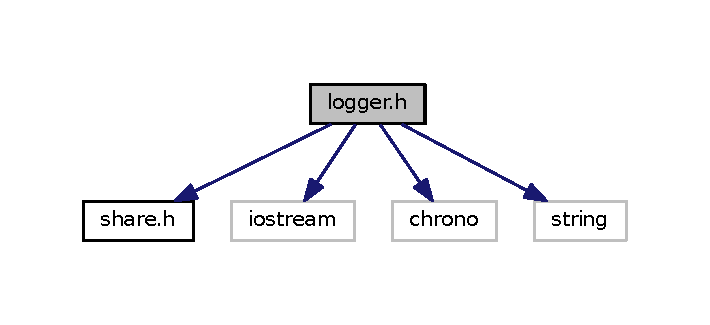
\includegraphics[width=341pt]{logger_8h__incl}
\end{center}
\end{figure}
\subsection*{Classes}
\begin{DoxyCompactItemize}
\item 
struct \hyperlink{struct_logger}{Logger}
\end{DoxyCompactItemize}

\hypertarget{main_8cpp}{}\section{main.\+cpp File Reference}
\label{main_8cpp}\index{main.\+cpp@{main.\+cpp}}
{\ttfamily \#include \char`\"{}share.\+h\char`\"{}}\\*
{\ttfamily \#include $<$iostream$>$}\\*
{\ttfamily \#include \char`\"{}print\+\_\+ip.\+h\char`\"{}}\\*
Include dependency graph for main.\+cpp\+:
\nopagebreak
\begin{figure}[H]
\begin{center}
\leavevmode
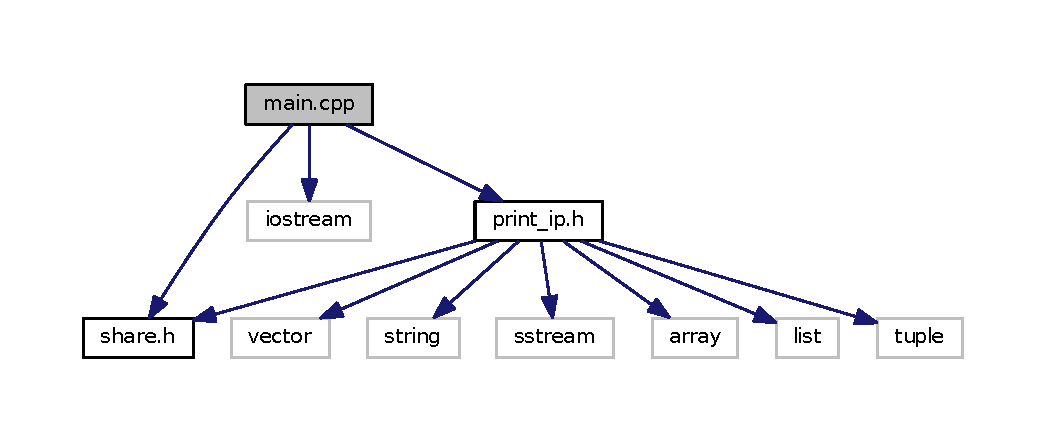
\includegraphics[width=350pt]{main_8cpp__incl}
\end{center}
\end{figure}
\subsection*{Functions}
\begin{DoxyCompactItemize}
\item 
int \hyperlink{main_8cpp_ae66f6b31b5ad750f1fe042a706a4e3d4}{main} ()
\end{DoxyCompactItemize}


\subsection{Function Documentation}
\index{main.\+cpp@{main.\+cpp}!main@{main}}
\index{main@{main}!main.\+cpp@{main.\+cpp}}
\subsubsection[{\texorpdfstring{main()}{main()}}]{\setlength{\rightskip}{0pt plus 5cm}int main (
\begin{DoxyParamCaption}
{}
\end{DoxyParamCaption}
)}\hypertarget{main_8cpp_ae66f6b31b5ad750f1fe042a706a4e3d4}{}\label{main_8cpp_ae66f6b31b5ad750f1fe042a706a4e3d4}


Definition at line 10 of file main.\+cpp.



Here is the call graph for this function\+:
\nopagebreak
\begin{figure}[H]
\begin{center}
\leavevmode
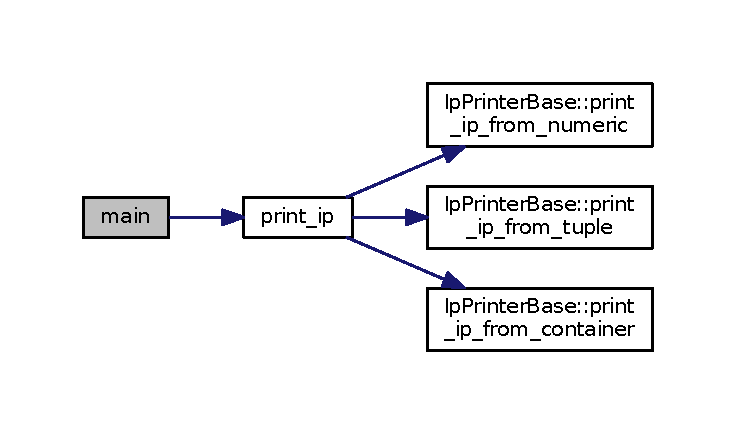
\includegraphics[width=350pt]{main_8cpp_ae66f6b31b5ad750f1fe042a706a4e3d4_cgraph}
\end{center}
\end{figure}



\hypertarget{print__ip_8h}{}\section{print\+\_\+ip.\+h File Reference}
\label{print__ip_8h}\index{print\+\_\+ip.\+h@{print\+\_\+ip.\+h}}
{\ttfamily \#include \char`\"{}share.\+h\char`\"{}}\\*
{\ttfamily \#include $<$vector$>$}\\*
{\ttfamily \#include $<$string$>$}\\*
{\ttfamily \#include $<$sstream$>$}\\*
{\ttfamily \#include $<$array$>$}\\*
{\ttfamily \#include $<$list$>$}\\*
{\ttfamily \#include $<$tuple$>$}\\*
Include dependency graph for print\+\_\+ip.\+h\+:
\nopagebreak
\begin{figure}[H]
\begin{center}
\leavevmode
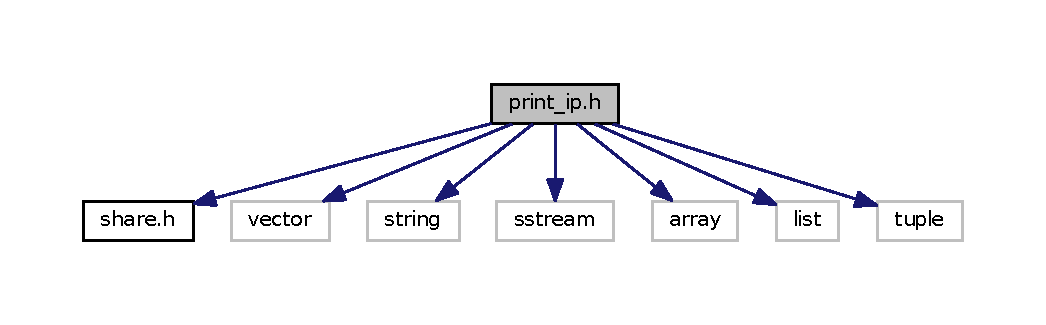
\includegraphics[width=350pt]{print__ip_8h__incl}
\end{center}
\end{figure}
This graph shows which files directly or indirectly include this file\+:
\nopagebreak
\begin{figure}[H]
\begin{center}
\leavevmode
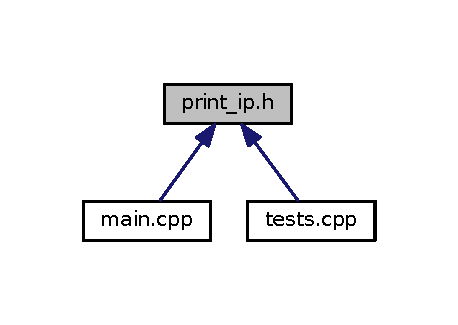
\includegraphics[width=220pt]{print__ip_8h__dep__incl}
\end{center}
\end{figure}
\subsection*{Classes}
\begin{DoxyCompactItemize}
\item 
struct \hyperlink{structis__specialization__of}{is\+\_\+specialization\+\_\+of$<$ Template, T $>$}
\item 
struct \hyperlink{structis__specialization__of_3_01_template_00_01_template_3_01_args_8_8_8_01_4_01_4}{is\+\_\+specialization\+\_\+of$<$ Template, Template$<$ Args... $>$ $>$}
\item 
struct \hyperlink{struct_ip_printer_base}{Ip\+Printer\+Base$<$ Derived $>$}
\item 
class \hyperlink{class_ip_printer}{Ip\+Printer}
\end{DoxyCompactItemize}
\subsection*{Functions}
\begin{DoxyCompactItemize}
\item 
{\footnotesize template$<$typename T $>$ }\\string \hyperlink{print__ip_8h_ae63874d29a9004ff5d4eaf4f7ca78393}{print\+\_\+ip} (const T \&ip)
\end{DoxyCompactItemize}
\subsection*{Variables}
\begin{DoxyCompactItemize}
\item 
{\footnotesize template$<$class \+\_\+\+Ty $>$ }\\constexpr bool \hyperlink{print__ip_8h_a396e4b8c756441b942c1619de108e56a}{is\+\_\+integral\+\_\+v} = std\+::is\+\_\+integral$<$\+\_\+\+Ty$>$\+::value
\item 
{\footnotesize template$<$class \+\_\+\+Ty1 , class \+\_\+\+Ty2 $>$ }\\constexpr bool \hyperlink{print__ip_8h_aa6c6bde5fd020a928e6d7b5fe8db7bb0}{is\+\_\+same\+\_\+v} = std\+::is\+\_\+same$<$\+\_\+\+Ty1, \+\_\+\+Ty2$>$\+::value
\item 
{\footnotesize template$<$class T $>$ }\\constexpr bool \hyperlink{print__ip_8h_a7f6f282ffeac81407489efbeee474dce}{is\+\_\+tuple\+\_\+v} = \hyperlink{structis__specialization__of}{is\+\_\+specialization\+\_\+of}$<$std\+::tuple, T$>$\+::value
\item 
{\footnotesize template$<$class T $>$ }\\constexpr bool \hyperlink{print__ip_8h_a4fbf025a5168661ab4054b8acf9221e9}{is\+\_\+vector\+\_\+v} = \hyperlink{structis__specialization__of}{is\+\_\+specialization\+\_\+of}$<$std\+::vector, T$>$\+::value
\item 
{\footnotesize template$<$class T $>$ }\\constexpr bool \hyperlink{print__ip_8h_aba616383699ab0a96098de59a81b9c89}{is\+\_\+list\+\_\+v} = \hyperlink{structis__specialization__of}{is\+\_\+specialization\+\_\+of}$<$std\+::list, T$>$\+::value
\end{DoxyCompactItemize}


\subsection{Function Documentation}
\index{print\+\_\+ip.\+h@{print\+\_\+ip.\+h}!print\+\_\+ip@{print\+\_\+ip}}
\index{print\+\_\+ip@{print\+\_\+ip}!print\+\_\+ip.\+h@{print\+\_\+ip.\+h}}
\subsubsection[{\texorpdfstring{print\+\_\+ip(const T \&ip)}{print_ip(const T &ip)}}]{\setlength{\rightskip}{0pt plus 5cm}template$<$typename T $>$ string print\+\_\+ip (
\begin{DoxyParamCaption}
\item[{const T \&}]{ip}
\end{DoxyParamCaption}
)}\hypertarget{print__ip_8h_ae63874d29a9004ff5d4eaf4f7ca78393}{}\label{print__ip_8h_ae63874d29a9004ff5d4eaf4f7ca78393}


Definition at line 119 of file print\+\_\+ip.\+h.



Here is the call graph for this function\+:
\nopagebreak
\begin{figure}[H]
\begin{center}
\leavevmode
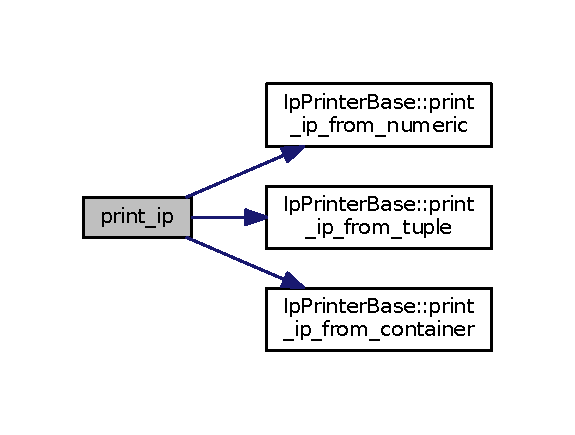
\includegraphics[width=276pt]{print__ip_8h_ae63874d29a9004ff5d4eaf4f7ca78393_cgraph}
\end{center}
\end{figure}




Here is the caller graph for this function\+:
\nopagebreak
\begin{figure}[H]
\begin{center}
\leavevmode
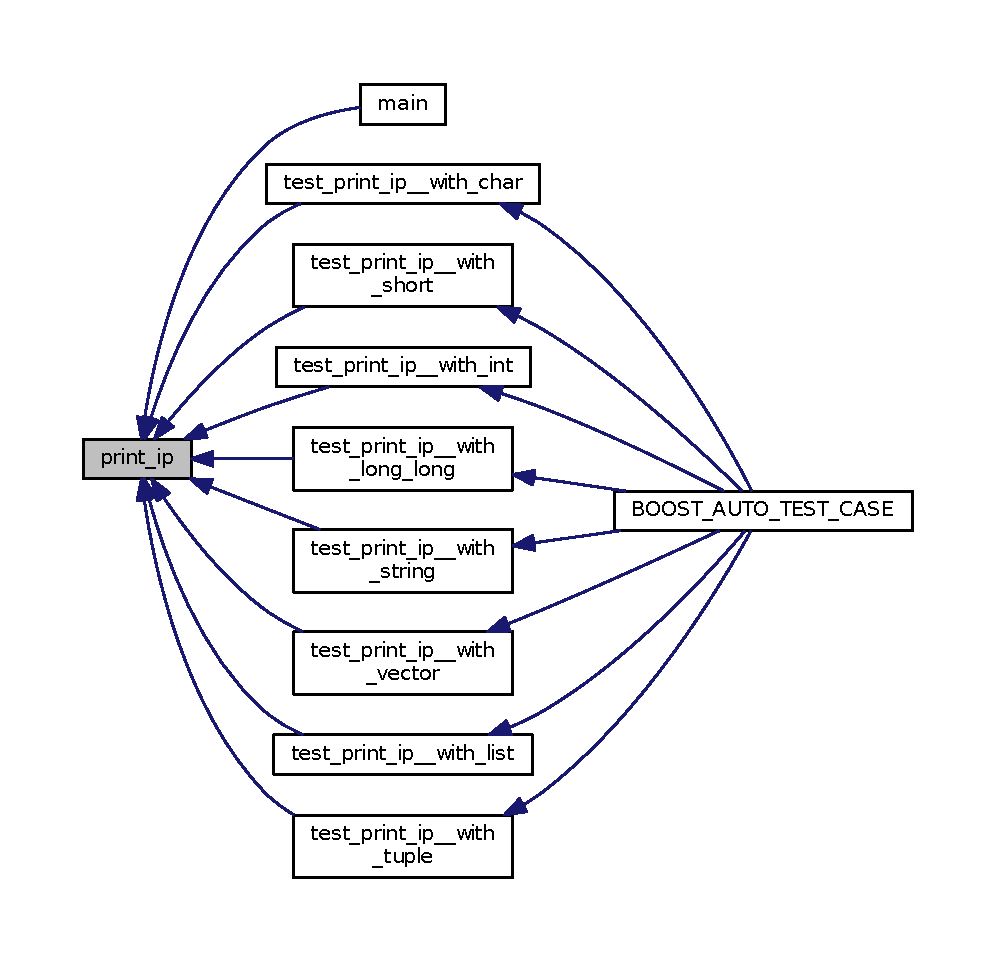
\includegraphics[width=350pt]{print__ip_8h_ae63874d29a9004ff5d4eaf4f7ca78393_icgraph}
\end{center}
\end{figure}




\subsection{Variable Documentation}
\index{print\+\_\+ip.\+h@{print\+\_\+ip.\+h}!is\+\_\+integral\+\_\+v@{is\+\_\+integral\+\_\+v}}
\index{is\+\_\+integral\+\_\+v@{is\+\_\+integral\+\_\+v}!print\+\_\+ip.\+h@{print\+\_\+ip.\+h}}
\subsubsection[{\texorpdfstring{is\+\_\+integral\+\_\+v}{is_integral_v}}]{\setlength{\rightskip}{0pt plus 5cm}template$<$class \+\_\+\+Ty $>$ constexpr bool is\+\_\+integral\+\_\+v = std\+::is\+\_\+integral$<$\+\_\+\+Ty$>$\+::value}\hypertarget{print__ip_8h_a396e4b8c756441b942c1619de108e56a}{}\label{print__ip_8h_a396e4b8c756441b942c1619de108e56a}


Definition at line 17 of file print\+\_\+ip.\+h.

\index{print\+\_\+ip.\+h@{print\+\_\+ip.\+h}!is\+\_\+list\+\_\+v@{is\+\_\+list\+\_\+v}}
\index{is\+\_\+list\+\_\+v@{is\+\_\+list\+\_\+v}!print\+\_\+ip.\+h@{print\+\_\+ip.\+h}}
\subsubsection[{\texorpdfstring{is\+\_\+list\+\_\+v}{is_list_v}}]{\setlength{\rightskip}{0pt plus 5cm}template$<$class T $>$ constexpr bool is\+\_\+list\+\_\+v = {\bf is\+\_\+specialization\+\_\+of}$<$std\+::list, T$>$\+::value}\hypertarget{print__ip_8h_aba616383699ab0a96098de59a81b9c89}{}\label{print__ip_8h_aba616383699ab0a96098de59a81b9c89}


Definition at line 35 of file print\+\_\+ip.\+h.

\index{print\+\_\+ip.\+h@{print\+\_\+ip.\+h}!is\+\_\+same\+\_\+v@{is\+\_\+same\+\_\+v}}
\index{is\+\_\+same\+\_\+v@{is\+\_\+same\+\_\+v}!print\+\_\+ip.\+h@{print\+\_\+ip.\+h}}
\subsubsection[{\texorpdfstring{is\+\_\+same\+\_\+v}{is_same_v}}]{\setlength{\rightskip}{0pt plus 5cm}template$<$class \+\_\+\+Ty1 , class \+\_\+\+Ty2 $>$ constexpr bool is\+\_\+same\+\_\+v = std\+::is\+\_\+same$<$\+\_\+\+Ty1, \+\_\+\+Ty2$>$\+::value}\hypertarget{print__ip_8h_aa6c6bde5fd020a928e6d7b5fe8db7bb0}{}\label{print__ip_8h_aa6c6bde5fd020a928e6d7b5fe8db7bb0}


Definition at line 20 of file print\+\_\+ip.\+h.

\index{print\+\_\+ip.\+h@{print\+\_\+ip.\+h}!is\+\_\+tuple\+\_\+v@{is\+\_\+tuple\+\_\+v}}
\index{is\+\_\+tuple\+\_\+v@{is\+\_\+tuple\+\_\+v}!print\+\_\+ip.\+h@{print\+\_\+ip.\+h}}
\subsubsection[{\texorpdfstring{is\+\_\+tuple\+\_\+v}{is_tuple_v}}]{\setlength{\rightskip}{0pt plus 5cm}template$<$class T $>$ constexpr bool is\+\_\+tuple\+\_\+v = {\bf is\+\_\+specialization\+\_\+of}$<$std\+::tuple, T$>$\+::value}\hypertarget{print__ip_8h_a7f6f282ffeac81407489efbeee474dce}{}\label{print__ip_8h_a7f6f282ffeac81407489efbeee474dce}


Definition at line 29 of file print\+\_\+ip.\+h.

\index{print\+\_\+ip.\+h@{print\+\_\+ip.\+h}!is\+\_\+vector\+\_\+v@{is\+\_\+vector\+\_\+v}}
\index{is\+\_\+vector\+\_\+v@{is\+\_\+vector\+\_\+v}!print\+\_\+ip.\+h@{print\+\_\+ip.\+h}}
\subsubsection[{\texorpdfstring{is\+\_\+vector\+\_\+v}{is_vector_v}}]{\setlength{\rightskip}{0pt plus 5cm}template$<$class T $>$ constexpr bool is\+\_\+vector\+\_\+v = {\bf is\+\_\+specialization\+\_\+of}$<$std\+::vector, T$>$\+::value}\hypertarget{print__ip_8h_a4fbf025a5168661ab4054b8acf9221e9}{}\label{print__ip_8h_a4fbf025a5168661ab4054b8acf9221e9}


Definition at line 32 of file print\+\_\+ip.\+h.


\hypertarget{share_8h}{}\section{share.\+h File Reference}
\label{share_8h}\index{share.\+h@{share.\+h}}
This graph shows which files directly or indirectly include this file\+:
\nopagebreak
\begin{figure}[H]
\begin{center}
\leavevmode
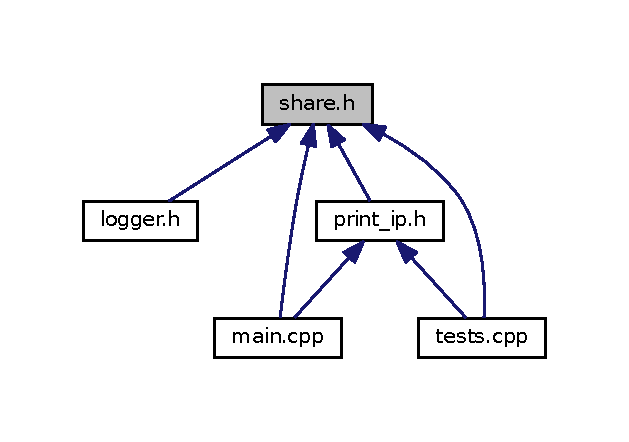
\includegraphics[width=302pt]{share_8h__dep__incl}
\end{center}
\end{figure}

\hypertarget{tests_8cpp}{}\section{tests.\+cpp File Reference}
\label{tests_8cpp}\index{tests.\+cpp@{tests.\+cpp}}
{\ttfamily \#include \char`\"{}share.\+h\char`\"{}}\\*
{\ttfamily \#include $<$boost/test/unit\+\_\+test.\+hpp$>$}\\*
{\ttfamily \#include $<$iostream$>$}\\*
{\ttfamily \#include $<$functional$>$}\\*
{\ttfamily \#include $<$ctime$>$}\\*
{\ttfamily \#include $<$tuple$>$}\\*
{\ttfamily \#include \char`\"{}print\+\_\+ip.\+h\char`\"{}}\\*
Include dependency graph for tests.\+cpp\+:
\nopagebreak
\begin{figure}[H]
\begin{center}
\leavevmode
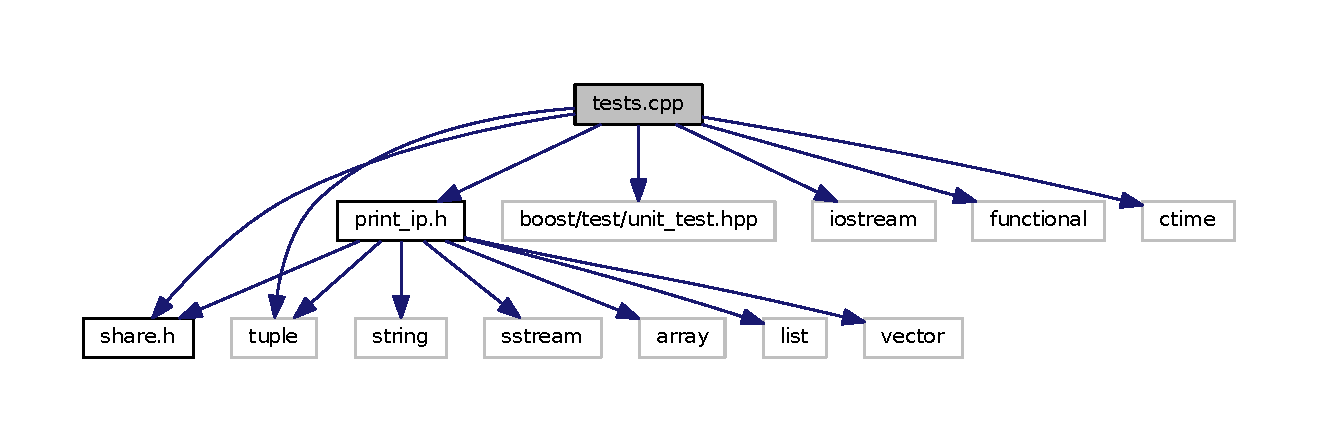
\includegraphics[width=350pt]{tests_8cpp__incl}
\end{center}
\end{figure}
\subsection*{Macros}
\begin{DoxyCompactItemize}
\item 
\#define \hyperlink{tests_8cpp_a6b2a3852db8bb19ab6909bac01859985}{B\+O\+O\+S\+T\+\_\+\+T\+E\+S\+T\+\_\+\+M\+O\+D\+U\+LE}~allocator\+\_\+test\+\_\+module
\end{DoxyCompactItemize}
\subsection*{Functions}
\begin{DoxyCompactItemize}
\item 
bool \hyperlink{tests_8cpp_aa077d5d13677e8627ef4bb67164ec979}{call\+\_\+test} (string name, std\+::function$<$ bool(void)$>$ fntest)
\item 
bool \hyperlink{tests_8cpp_a819cf6bf1d1705e50ca118e1b9185016}{test\+\_\+print\+\_\+ip\+\_\+\+\_\+with\+\_\+char} ()
\item 
bool \hyperlink{tests_8cpp_ad947862d2313baa3355ad397472f963d}{test\+\_\+print\+\_\+ip\+\_\+\+\_\+with\+\_\+short} ()
\item 
bool \hyperlink{tests_8cpp_a39d34ef8a0250c73cb3b6009e98adc39}{test\+\_\+print\+\_\+ip\+\_\+\+\_\+with\+\_\+int} ()
\item 
bool \hyperlink{tests_8cpp_ab8e03bbc20567765d83c7ca439d1fc4e}{test\+\_\+print\+\_\+ip\+\_\+\+\_\+with\+\_\+long\+\_\+long} ()
\item 
bool \hyperlink{tests_8cpp_aa9f9e2e14338ae5d9d01430fe949dc99}{test\+\_\+print\+\_\+ip\+\_\+\+\_\+with\+\_\+string} ()
\item 
bool \hyperlink{tests_8cpp_a6603188be27664b95cf696eb246623a6}{test\+\_\+print\+\_\+ip\+\_\+\+\_\+with\+\_\+vector} ()
\item 
bool \hyperlink{tests_8cpp_a638d1801c86c2c8c06dac2f61b290277}{test\+\_\+print\+\_\+ip\+\_\+\+\_\+with\+\_\+list} ()
\item 
bool \hyperlink{tests_8cpp_a3445971afb7200d66b90472ad0460a81}{test\+\_\+print\+\_\+ip\+\_\+\+\_\+with\+\_\+tuple} ()
\item 
\hyperlink{tests_8cpp_a70ab11e47ed9d11226eba2bfd0a40115}{B\+O\+O\+S\+T\+\_\+\+A\+U\+T\+O\+\_\+\+T\+E\+S\+T\+\_\+\+C\+A\+SE} (test\+\_\+of\+\_\+print\+\_\+ip)
\end{DoxyCompactItemize}


\subsection{Macro Definition Documentation}
\index{tests.\+cpp@{tests.\+cpp}!B\+O\+O\+S\+T\+\_\+\+T\+E\+S\+T\+\_\+\+M\+O\+D\+U\+LE@{B\+O\+O\+S\+T\+\_\+\+T\+E\+S\+T\+\_\+\+M\+O\+D\+U\+LE}}
\index{B\+O\+O\+S\+T\+\_\+\+T\+E\+S\+T\+\_\+\+M\+O\+D\+U\+LE@{B\+O\+O\+S\+T\+\_\+\+T\+E\+S\+T\+\_\+\+M\+O\+D\+U\+LE}!tests.\+cpp@{tests.\+cpp}}
\subsubsection[{\texorpdfstring{B\+O\+O\+S\+T\+\_\+\+T\+E\+S\+T\+\_\+\+M\+O\+D\+U\+LE}{BOOST_TEST_MODULE}}]{\setlength{\rightskip}{0pt plus 5cm}\#define B\+O\+O\+S\+T\+\_\+\+T\+E\+S\+T\+\_\+\+M\+O\+D\+U\+LE~allocator\+\_\+test\+\_\+module}\hypertarget{tests_8cpp_a6b2a3852db8bb19ab6909bac01859985}{}\label{tests_8cpp_a6b2a3852db8bb19ab6909bac01859985}


Definition at line 3 of file tests.\+cpp.



\subsection{Function Documentation}
\index{tests.\+cpp@{tests.\+cpp}!B\+O\+O\+S\+T\+\_\+\+A\+U\+T\+O\+\_\+\+T\+E\+S\+T\+\_\+\+C\+A\+SE@{B\+O\+O\+S\+T\+\_\+\+A\+U\+T\+O\+\_\+\+T\+E\+S\+T\+\_\+\+C\+A\+SE}}
\index{B\+O\+O\+S\+T\+\_\+\+A\+U\+T\+O\+\_\+\+T\+E\+S\+T\+\_\+\+C\+A\+SE@{B\+O\+O\+S\+T\+\_\+\+A\+U\+T\+O\+\_\+\+T\+E\+S\+T\+\_\+\+C\+A\+SE}!tests.\+cpp@{tests.\+cpp}}
\subsubsection[{\texorpdfstring{B\+O\+O\+S\+T\+\_\+\+A\+U\+T\+O\+\_\+\+T\+E\+S\+T\+\_\+\+C\+A\+S\+E(test\+\_\+of\+\_\+print\+\_\+ip)}{BOOST_AUTO_TEST_CASE(test_of_print_ip)}}]{\setlength{\rightskip}{0pt plus 5cm}B\+O\+O\+S\+T\+\_\+\+A\+U\+T\+O\+\_\+\+T\+E\+S\+T\+\_\+\+C\+A\+SE (
\begin{DoxyParamCaption}
\item[{test\+\_\+of\+\_\+print\+\_\+ip}]{}
\end{DoxyParamCaption}
)}\hypertarget{tests_8cpp_a70ab11e47ed9d11226eba2bfd0a40115}{}\label{tests_8cpp_a70ab11e47ed9d11226eba2bfd0a40115}


Definition at line 88 of file tests.\+cpp.



Here is the call graph for this function\+:
\nopagebreak
\begin{figure}[H]
\begin{center}
\leavevmode
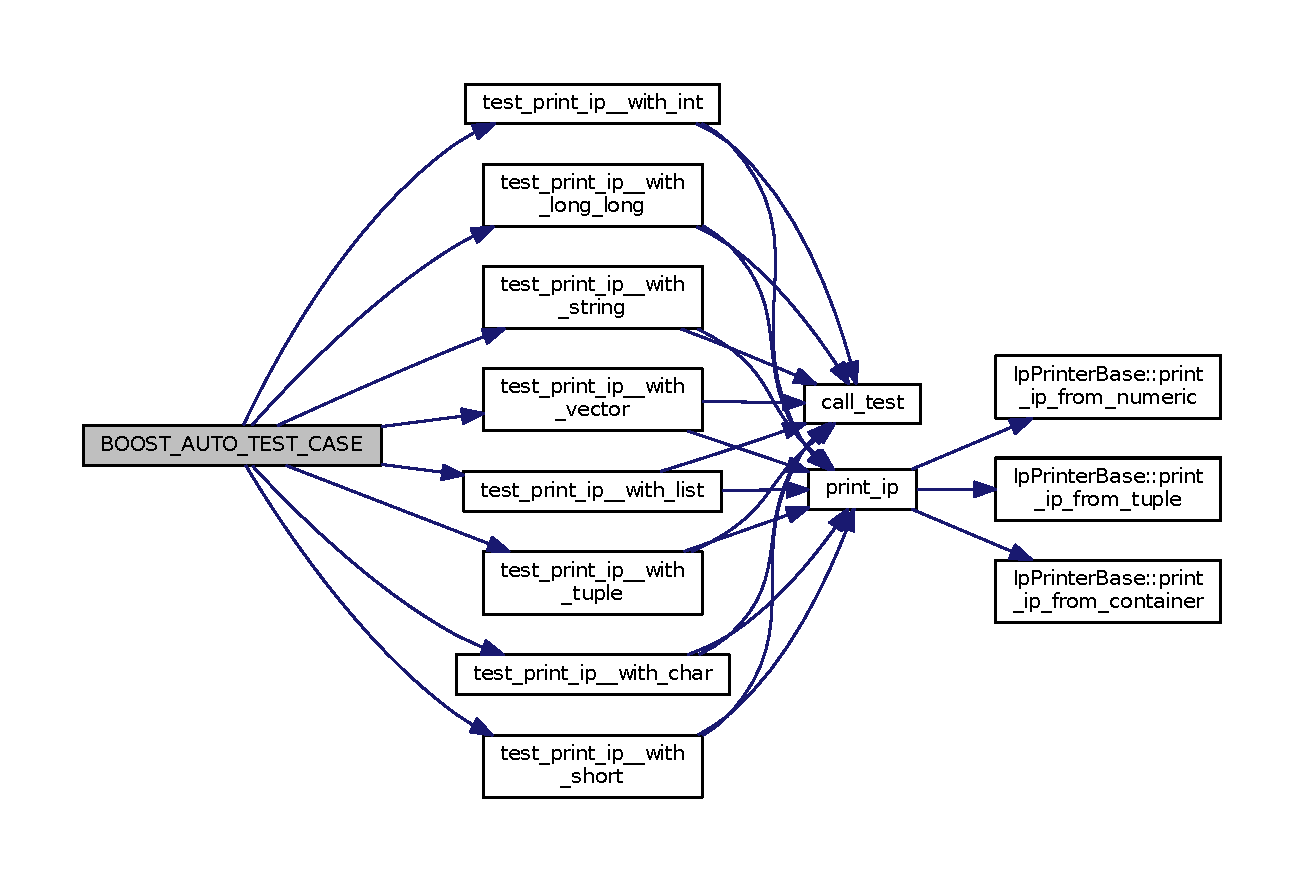
\includegraphics[width=350pt]{tests_8cpp_a70ab11e47ed9d11226eba2bfd0a40115_cgraph}
\end{center}
\end{figure}


\index{tests.\+cpp@{tests.\+cpp}!call\+\_\+test@{call\+\_\+test}}
\index{call\+\_\+test@{call\+\_\+test}!tests.\+cpp@{tests.\+cpp}}
\subsubsection[{\texorpdfstring{call\+\_\+test(string name, std\+::function$<$ bool(void)$>$ fntest)}{call_test(string name, std::function< bool(void)> fntest)}}]{\setlength{\rightskip}{0pt plus 5cm}bool call\+\_\+test (
\begin{DoxyParamCaption}
\item[{string}]{name, }
\item[{std\+::function$<$ bool(void)$>$}]{fntest}
\end{DoxyParamCaption}
)}\hypertarget{tests_8cpp_aa077d5d13677e8627ef4bb67164ec979}{}\label{tests_8cpp_aa077d5d13677e8627ef4bb67164ec979}


Definition at line 18 of file tests.\+cpp.



Here is the caller graph for this function\+:
\nopagebreak
\begin{figure}[H]
\begin{center}
\leavevmode
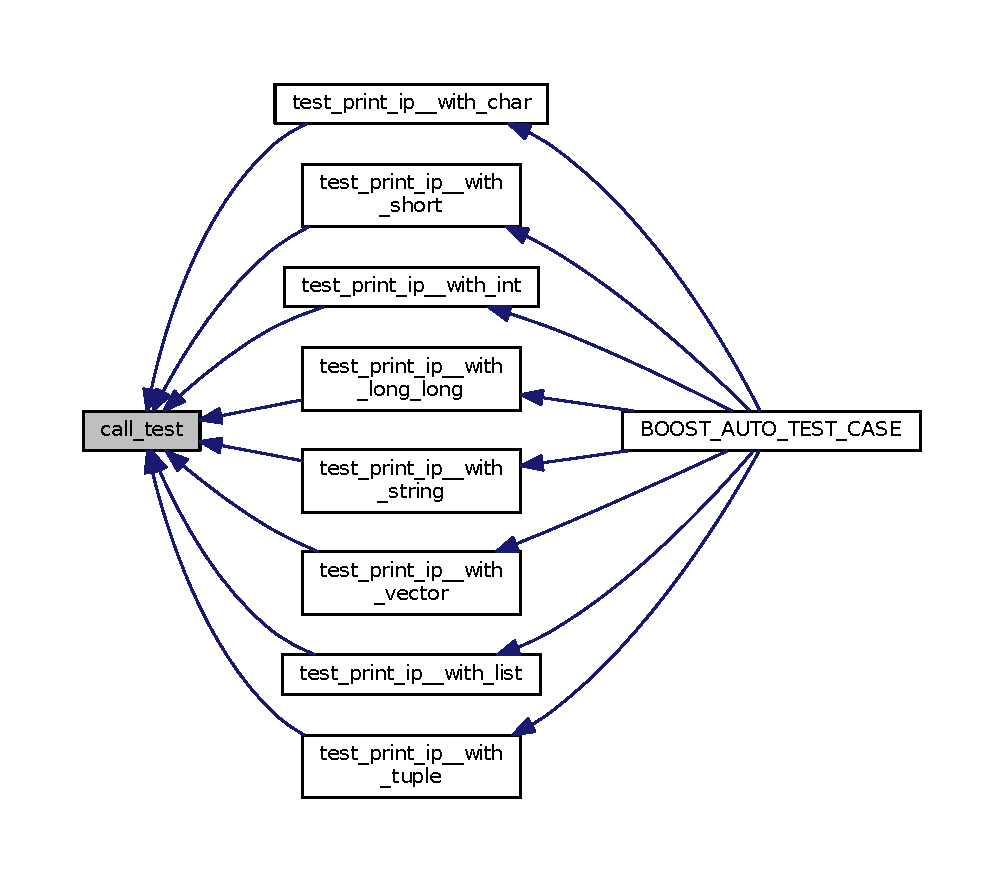
\includegraphics[width=350pt]{tests_8cpp_aa077d5d13677e8627ef4bb67164ec979_icgraph}
\end{center}
\end{figure}


\index{tests.\+cpp@{tests.\+cpp}!test\+\_\+print\+\_\+ip\+\_\+\+\_\+with\+\_\+char@{test\+\_\+print\+\_\+ip\+\_\+\+\_\+with\+\_\+char}}
\index{test\+\_\+print\+\_\+ip\+\_\+\+\_\+with\+\_\+char@{test\+\_\+print\+\_\+ip\+\_\+\+\_\+with\+\_\+char}!tests.\+cpp@{tests.\+cpp}}
\subsubsection[{\texorpdfstring{test\+\_\+print\+\_\+ip\+\_\+\+\_\+with\+\_\+char()}{test_print_ip__with_char()}}]{\setlength{\rightskip}{0pt plus 5cm}bool test\+\_\+print\+\_\+ip\+\_\+\+\_\+with\+\_\+char (
\begin{DoxyParamCaption}
{}
\end{DoxyParamCaption}
)}\hypertarget{tests_8cpp_a819cf6bf1d1705e50ca118e1b9185016}{}\label{tests_8cpp_a819cf6bf1d1705e50ca118e1b9185016}


Definition at line 29 of file tests.\+cpp.



Here is the call graph for this function\+:
\nopagebreak
\begin{figure}[H]
\begin{center}
\leavevmode
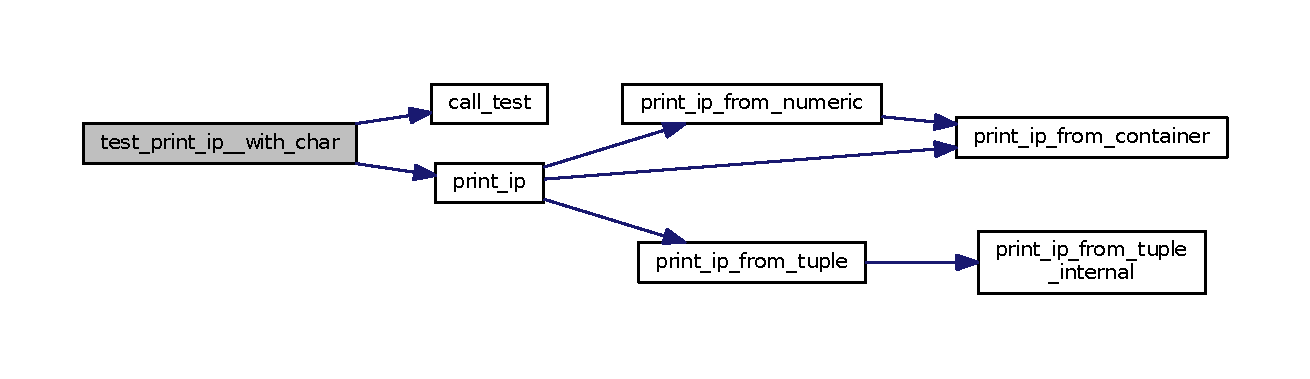
\includegraphics[width=350pt]{tests_8cpp_a819cf6bf1d1705e50ca118e1b9185016_cgraph}
\end{center}
\end{figure}




Here is the caller graph for this function\+:
\nopagebreak
\begin{figure}[H]
\begin{center}
\leavevmode
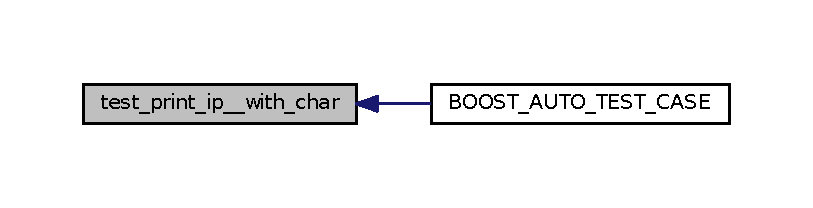
\includegraphics[width=350pt]{tests_8cpp_a819cf6bf1d1705e50ca118e1b9185016_icgraph}
\end{center}
\end{figure}


\index{tests.\+cpp@{tests.\+cpp}!test\+\_\+print\+\_\+ip\+\_\+\+\_\+with\+\_\+int@{test\+\_\+print\+\_\+ip\+\_\+\+\_\+with\+\_\+int}}
\index{test\+\_\+print\+\_\+ip\+\_\+\+\_\+with\+\_\+int@{test\+\_\+print\+\_\+ip\+\_\+\+\_\+with\+\_\+int}!tests.\+cpp@{tests.\+cpp}}
\subsubsection[{\texorpdfstring{test\+\_\+print\+\_\+ip\+\_\+\+\_\+with\+\_\+int()}{test_print_ip__with_int()}}]{\setlength{\rightskip}{0pt plus 5cm}bool test\+\_\+print\+\_\+ip\+\_\+\+\_\+with\+\_\+int (
\begin{DoxyParamCaption}
{}
\end{DoxyParamCaption}
)}\hypertarget{tests_8cpp_a39d34ef8a0250c73cb3b6009e98adc39}{}\label{tests_8cpp_a39d34ef8a0250c73cb3b6009e98adc39}


Definition at line 41 of file tests.\+cpp.



Here is the call graph for this function\+:
\nopagebreak
\begin{figure}[H]
\begin{center}
\leavevmode
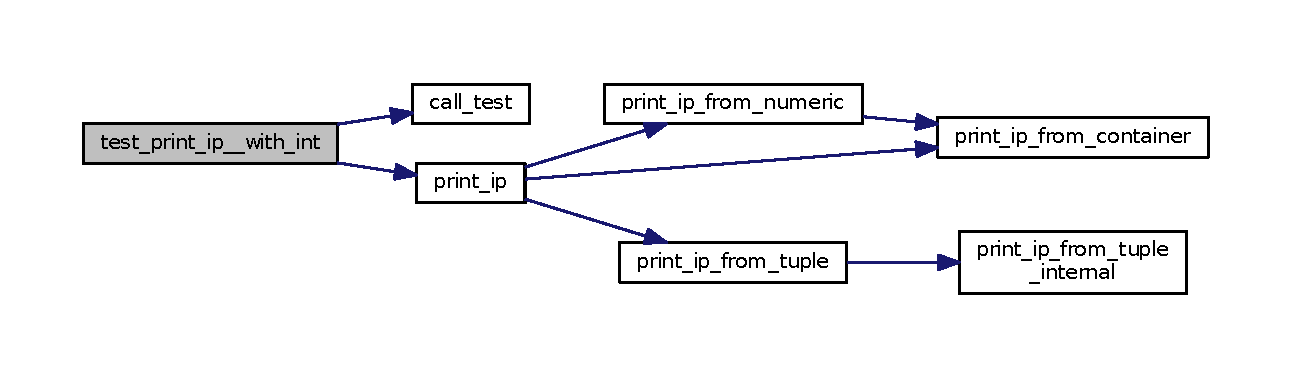
\includegraphics[width=350pt]{tests_8cpp_a39d34ef8a0250c73cb3b6009e98adc39_cgraph}
\end{center}
\end{figure}




Here is the caller graph for this function\+:
\nopagebreak
\begin{figure}[H]
\begin{center}
\leavevmode
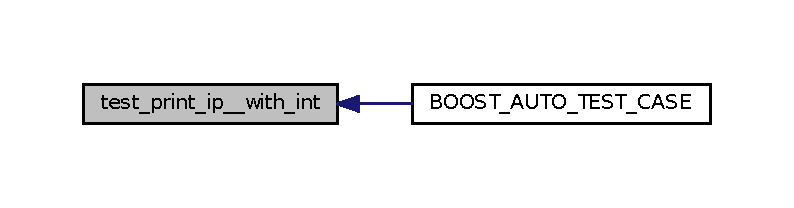
\includegraphics[width=350pt]{tests_8cpp_a39d34ef8a0250c73cb3b6009e98adc39_icgraph}
\end{center}
\end{figure}


\index{tests.\+cpp@{tests.\+cpp}!test\+\_\+print\+\_\+ip\+\_\+\+\_\+with\+\_\+list@{test\+\_\+print\+\_\+ip\+\_\+\+\_\+with\+\_\+list}}
\index{test\+\_\+print\+\_\+ip\+\_\+\+\_\+with\+\_\+list@{test\+\_\+print\+\_\+ip\+\_\+\+\_\+with\+\_\+list}!tests.\+cpp@{tests.\+cpp}}
\subsubsection[{\texorpdfstring{test\+\_\+print\+\_\+ip\+\_\+\+\_\+with\+\_\+list()}{test_print_ip__with_list()}}]{\setlength{\rightskip}{0pt plus 5cm}bool test\+\_\+print\+\_\+ip\+\_\+\+\_\+with\+\_\+list (
\begin{DoxyParamCaption}
{}
\end{DoxyParamCaption}
)}\hypertarget{tests_8cpp_a638d1801c86c2c8c06dac2f61b290277}{}\label{tests_8cpp_a638d1801c86c2c8c06dac2f61b290277}


Definition at line 65 of file tests.\+cpp.



Here is the call graph for this function\+:
\nopagebreak
\begin{figure}[H]
\begin{center}
\leavevmode
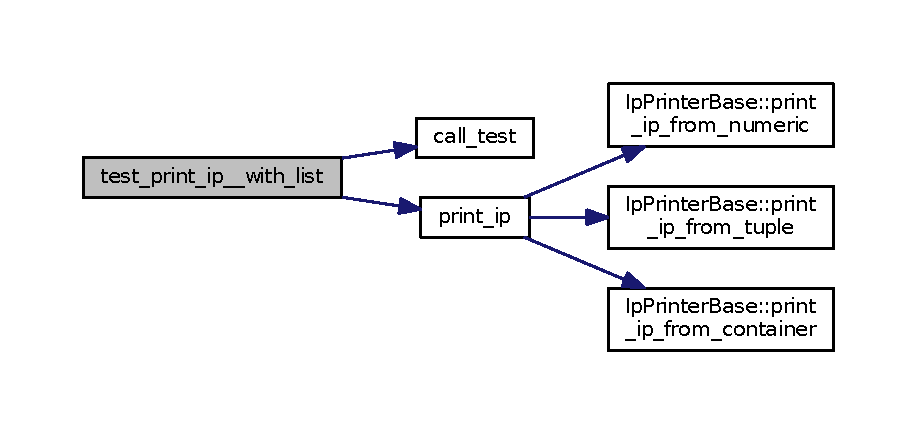
\includegraphics[width=350pt]{tests_8cpp_a638d1801c86c2c8c06dac2f61b290277_cgraph}
\end{center}
\end{figure}




Here is the caller graph for this function\+:
\nopagebreak
\begin{figure}[H]
\begin{center}
\leavevmode
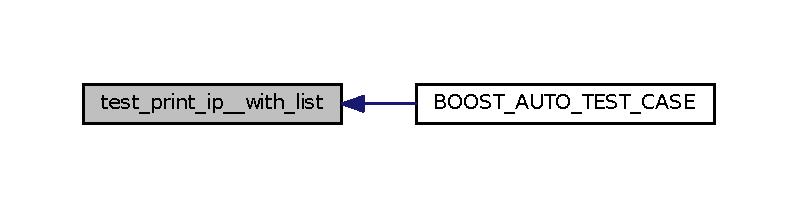
\includegraphics[width=350pt]{tests_8cpp_a638d1801c86c2c8c06dac2f61b290277_icgraph}
\end{center}
\end{figure}


\index{tests.\+cpp@{tests.\+cpp}!test\+\_\+print\+\_\+ip\+\_\+\+\_\+with\+\_\+long\+\_\+long@{test\+\_\+print\+\_\+ip\+\_\+\+\_\+with\+\_\+long\+\_\+long}}
\index{test\+\_\+print\+\_\+ip\+\_\+\+\_\+with\+\_\+long\+\_\+long@{test\+\_\+print\+\_\+ip\+\_\+\+\_\+with\+\_\+long\+\_\+long}!tests.\+cpp@{tests.\+cpp}}
\subsubsection[{\texorpdfstring{test\+\_\+print\+\_\+ip\+\_\+\+\_\+with\+\_\+long\+\_\+long()}{test_print_ip__with_long_long()}}]{\setlength{\rightskip}{0pt plus 5cm}bool test\+\_\+print\+\_\+ip\+\_\+\+\_\+with\+\_\+long\+\_\+long (
\begin{DoxyParamCaption}
{}
\end{DoxyParamCaption}
)}\hypertarget{tests_8cpp_ab8e03bbc20567765d83c7ca439d1fc4e}{}\label{tests_8cpp_ab8e03bbc20567765d83c7ca439d1fc4e}


Definition at line 47 of file tests.\+cpp.



Here is the call graph for this function\+:
\nopagebreak
\begin{figure}[H]
\begin{center}
\leavevmode
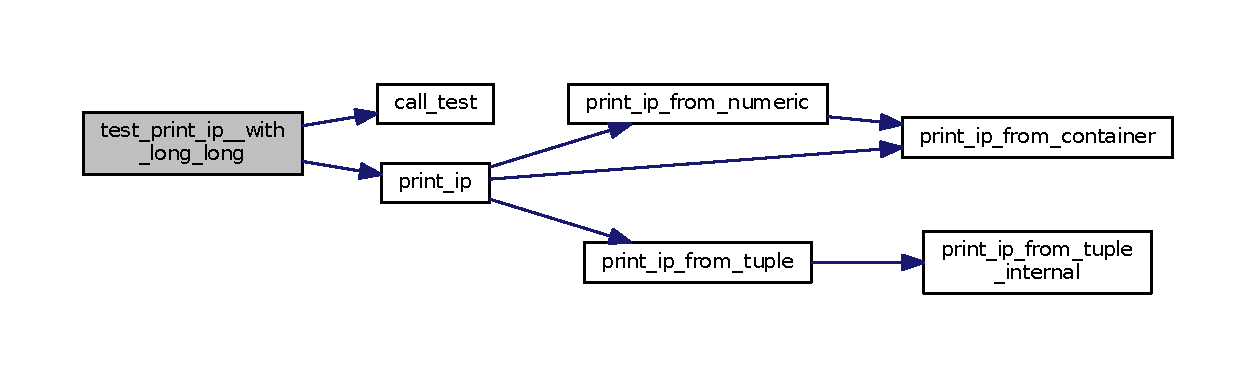
\includegraphics[width=350pt]{tests_8cpp_ab8e03bbc20567765d83c7ca439d1fc4e_cgraph}
\end{center}
\end{figure}




Here is the caller graph for this function\+:
\nopagebreak
\begin{figure}[H]
\begin{center}
\leavevmode
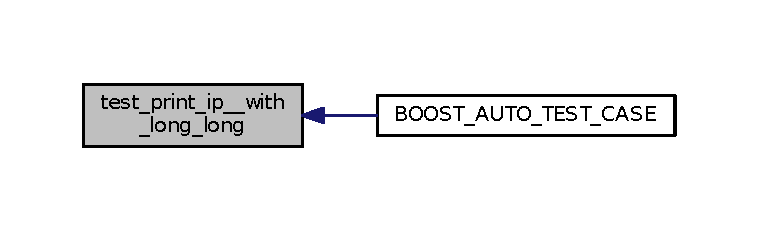
\includegraphics[width=350pt]{tests_8cpp_ab8e03bbc20567765d83c7ca439d1fc4e_icgraph}
\end{center}
\end{figure}


\index{tests.\+cpp@{tests.\+cpp}!test\+\_\+print\+\_\+ip\+\_\+\+\_\+with\+\_\+short@{test\+\_\+print\+\_\+ip\+\_\+\+\_\+with\+\_\+short}}
\index{test\+\_\+print\+\_\+ip\+\_\+\+\_\+with\+\_\+short@{test\+\_\+print\+\_\+ip\+\_\+\+\_\+with\+\_\+short}!tests.\+cpp@{tests.\+cpp}}
\subsubsection[{\texorpdfstring{test\+\_\+print\+\_\+ip\+\_\+\+\_\+with\+\_\+short()}{test_print_ip__with_short()}}]{\setlength{\rightskip}{0pt plus 5cm}bool test\+\_\+print\+\_\+ip\+\_\+\+\_\+with\+\_\+short (
\begin{DoxyParamCaption}
{}
\end{DoxyParamCaption}
)}\hypertarget{tests_8cpp_ad947862d2313baa3355ad397472f963d}{}\label{tests_8cpp_ad947862d2313baa3355ad397472f963d}


Definition at line 35 of file tests.\+cpp.



Here is the call graph for this function\+:
\nopagebreak
\begin{figure}[H]
\begin{center}
\leavevmode
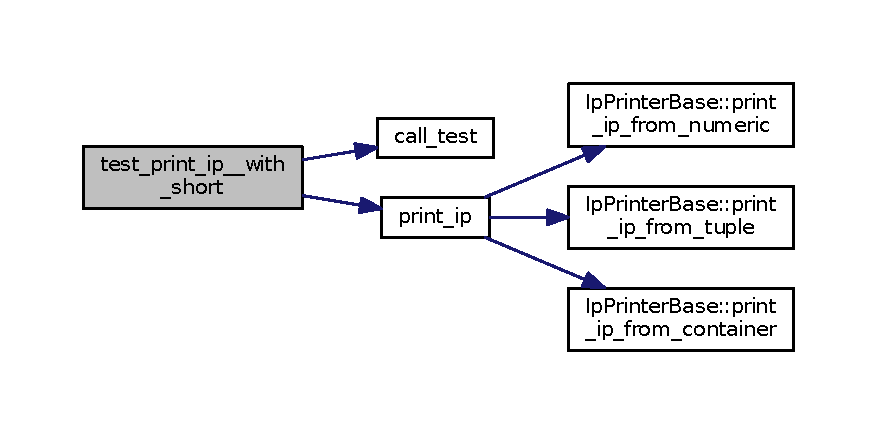
\includegraphics[width=350pt]{tests_8cpp_ad947862d2313baa3355ad397472f963d_cgraph}
\end{center}
\end{figure}




Here is the caller graph for this function\+:
\nopagebreak
\begin{figure}[H]
\begin{center}
\leavevmode
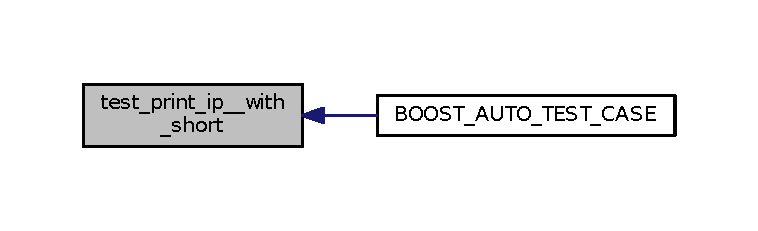
\includegraphics[width=350pt]{tests_8cpp_ad947862d2313baa3355ad397472f963d_icgraph}
\end{center}
\end{figure}


\index{tests.\+cpp@{tests.\+cpp}!test\+\_\+print\+\_\+ip\+\_\+\+\_\+with\+\_\+string@{test\+\_\+print\+\_\+ip\+\_\+\+\_\+with\+\_\+string}}
\index{test\+\_\+print\+\_\+ip\+\_\+\+\_\+with\+\_\+string@{test\+\_\+print\+\_\+ip\+\_\+\+\_\+with\+\_\+string}!tests.\+cpp@{tests.\+cpp}}
\subsubsection[{\texorpdfstring{test\+\_\+print\+\_\+ip\+\_\+\+\_\+with\+\_\+string()}{test_print_ip__with_string()}}]{\setlength{\rightskip}{0pt plus 5cm}bool test\+\_\+print\+\_\+ip\+\_\+\+\_\+with\+\_\+string (
\begin{DoxyParamCaption}
{}
\end{DoxyParamCaption}
)}\hypertarget{tests_8cpp_aa9f9e2e14338ae5d9d01430fe949dc99}{}\label{tests_8cpp_aa9f9e2e14338ae5d9d01430fe949dc99}


Definition at line 53 of file tests.\+cpp.



Here is the call graph for this function\+:
\nopagebreak
\begin{figure}[H]
\begin{center}
\leavevmode
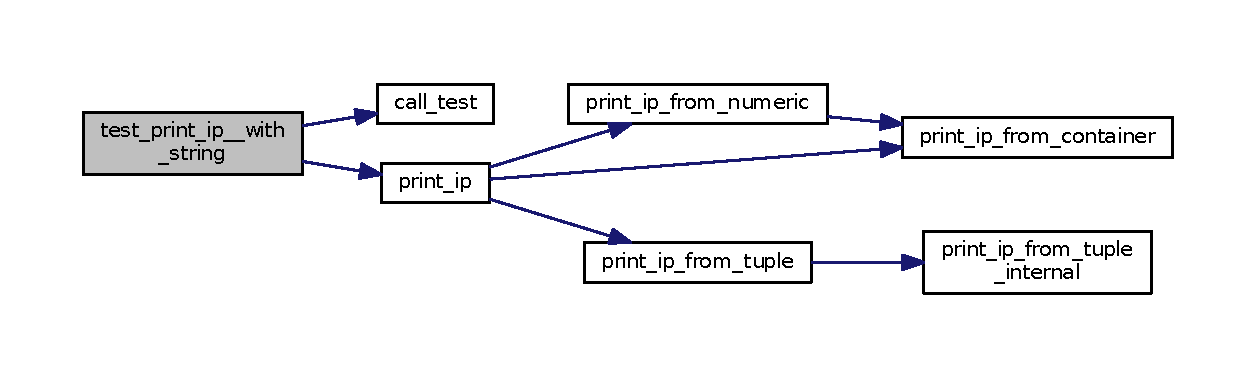
\includegraphics[width=350pt]{tests_8cpp_aa9f9e2e14338ae5d9d01430fe949dc99_cgraph}
\end{center}
\end{figure}




Here is the caller graph for this function\+:
\nopagebreak
\begin{figure}[H]
\begin{center}
\leavevmode
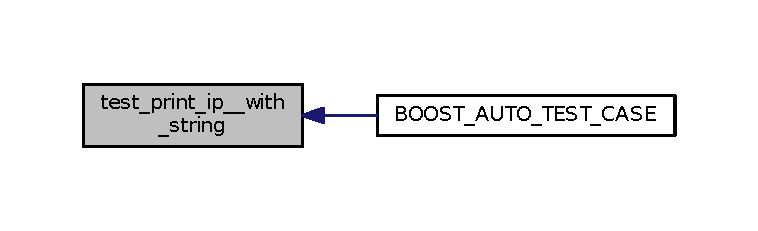
\includegraphics[width=350pt]{tests_8cpp_aa9f9e2e14338ae5d9d01430fe949dc99_icgraph}
\end{center}
\end{figure}


\index{tests.\+cpp@{tests.\+cpp}!test\+\_\+print\+\_\+ip\+\_\+\+\_\+with\+\_\+tuple@{test\+\_\+print\+\_\+ip\+\_\+\+\_\+with\+\_\+tuple}}
\index{test\+\_\+print\+\_\+ip\+\_\+\+\_\+with\+\_\+tuple@{test\+\_\+print\+\_\+ip\+\_\+\+\_\+with\+\_\+tuple}!tests.\+cpp@{tests.\+cpp}}
\subsubsection[{\texorpdfstring{test\+\_\+print\+\_\+ip\+\_\+\+\_\+with\+\_\+tuple()}{test_print_ip__with_tuple()}}]{\setlength{\rightskip}{0pt plus 5cm}bool test\+\_\+print\+\_\+ip\+\_\+\+\_\+with\+\_\+tuple (
\begin{DoxyParamCaption}
{}
\end{DoxyParamCaption}
)}\hypertarget{tests_8cpp_a3445971afb7200d66b90472ad0460a81}{}\label{tests_8cpp_a3445971afb7200d66b90472ad0460a81}


Definition at line 71 of file tests.\+cpp.



Here is the call graph for this function\+:
\nopagebreak
\begin{figure}[H]
\begin{center}
\leavevmode
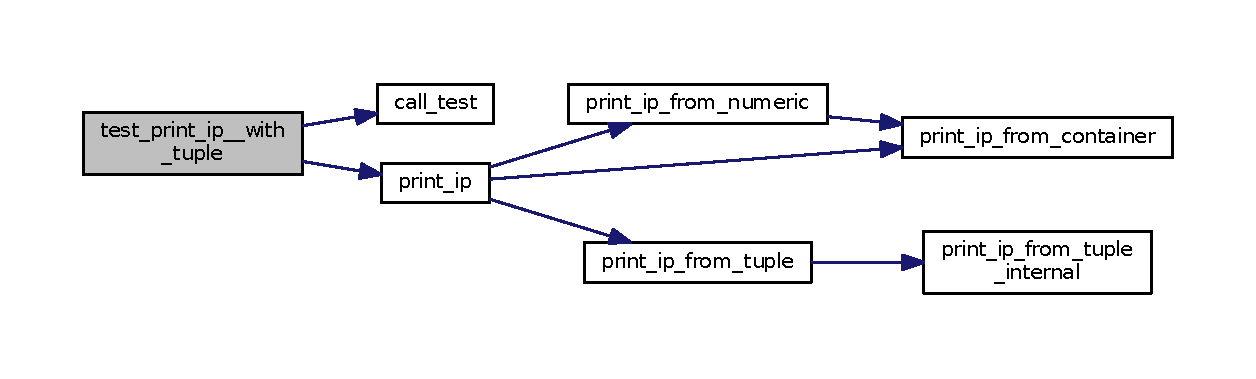
\includegraphics[width=350pt]{tests_8cpp_a3445971afb7200d66b90472ad0460a81_cgraph}
\end{center}
\end{figure}




Here is the caller graph for this function\+:
\nopagebreak
\begin{figure}[H]
\begin{center}
\leavevmode
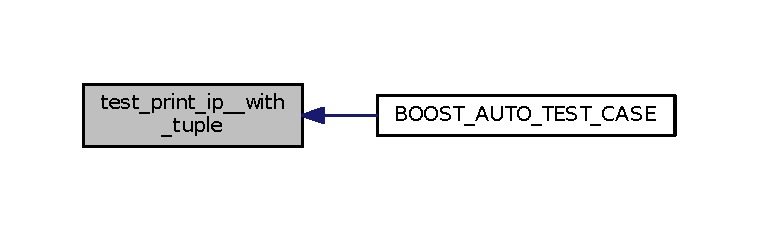
\includegraphics[width=350pt]{tests_8cpp_a3445971afb7200d66b90472ad0460a81_icgraph}
\end{center}
\end{figure}


\index{tests.\+cpp@{tests.\+cpp}!test\+\_\+print\+\_\+ip\+\_\+\+\_\+with\+\_\+vector@{test\+\_\+print\+\_\+ip\+\_\+\+\_\+with\+\_\+vector}}
\index{test\+\_\+print\+\_\+ip\+\_\+\+\_\+with\+\_\+vector@{test\+\_\+print\+\_\+ip\+\_\+\+\_\+with\+\_\+vector}!tests.\+cpp@{tests.\+cpp}}
\subsubsection[{\texorpdfstring{test\+\_\+print\+\_\+ip\+\_\+\+\_\+with\+\_\+vector()}{test_print_ip__with_vector()}}]{\setlength{\rightskip}{0pt plus 5cm}bool test\+\_\+print\+\_\+ip\+\_\+\+\_\+with\+\_\+vector (
\begin{DoxyParamCaption}
{}
\end{DoxyParamCaption}
)}\hypertarget{tests_8cpp_a6603188be27664b95cf696eb246623a6}{}\label{tests_8cpp_a6603188be27664b95cf696eb246623a6}


Definition at line 59 of file tests.\+cpp.



Here is the call graph for this function\+:
\nopagebreak
\begin{figure}[H]
\begin{center}
\leavevmode
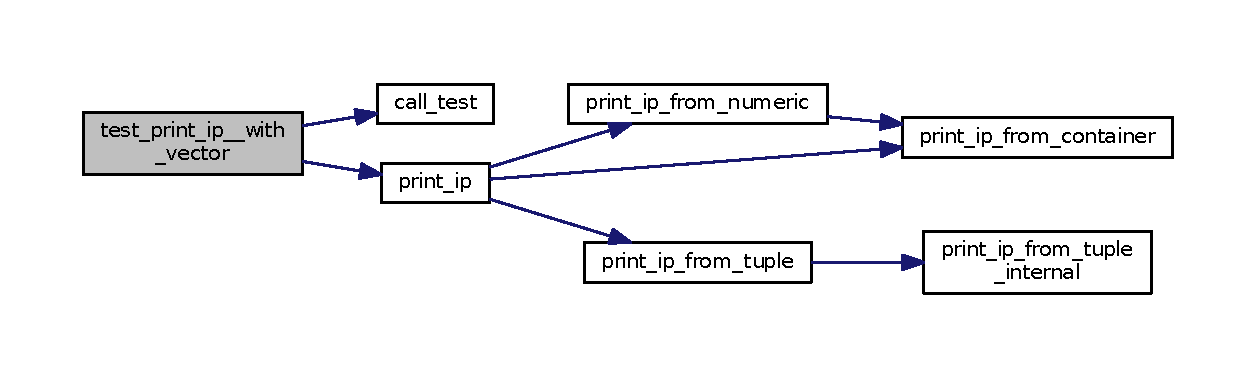
\includegraphics[width=350pt]{tests_8cpp_a6603188be27664b95cf696eb246623a6_cgraph}
\end{center}
\end{figure}




Here is the caller graph for this function\+:
\nopagebreak
\begin{figure}[H]
\begin{center}
\leavevmode
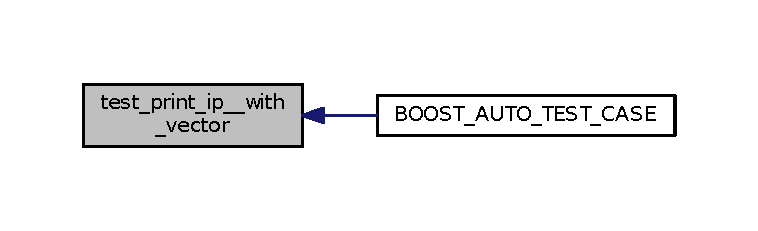
\includegraphics[width=350pt]{tests_8cpp_a6603188be27664b95cf696eb246623a6_icgraph}
\end{center}
\end{figure}



%--- End generated contents ---

% Index
\backmatter
\newpage
\phantomsection
\clearemptydoublepage
\addcontentsline{toc}{chapter}{Index}
\printindex

\end{document}
